\documentclass[9pt]{extarticle}
% Article
% \documentclass[9pt]{extarticle}
\usepackage[landscape, left=0.10cm, top=0.1cm, right=0.1cm, bottom=0.3cm, footskip=2pt]{geometry}
\usepackage{background}
\usepackage{etoolbox}
\usepackage{graphicx}
\usepackage{totcount}
\usepackage{lipsum}
\usepackage{hyperref}
\usepackage{amsmath}
\usepackage{amssymb}
\usepackage{physics}
\usepackage{enumerate}

\usepackage{xcolor}
\usepackage{tcolorbox}

\usepackage[compact]{titlesec}
\usepackage{paralist}

\usepackage{tabularx}
\usepackage{ctable}

% Set page margins

% Tables
\usepackage{tabularx, multirow}
\usepackage{booktabs}
\renewcommand*{\arraystretch}{2}

\def\BoxStart{\begin{tcolorbox}[colback=blue!5!white,colframe=blue!75!black]}
    \def\BoxEnd{\end{tcolorbox}}

% image directory
\graphicspath{ {./assets/} }

% For accessing arrays
\usepackage{etoolbox}

% for emumerating
\usepackage{enumitem}

% for color coding
\usetikzlibrary{backgrounds}

% for light font +C
\usepackage{color}
\definecolor{light}{rgb}{0.5, 0.5, 0.5}
\def\light#1{{\color{light}#1}}

% for multicolumn
\usepackage{multicol}
\setlength{\columnseprule}{0.4pt}

% to have access to the total number of subsection*s
%\regtotcounter{subsection*}

% every subsection* starts on a new page
%\pretocmd{\subsection*}{\clearpage}{}{}

% auxiliary lengths for the height of the frame and the width of each tab
\newlength\mylen{}
\newlength\mylena{}


\renewcommand*{\arraystretch}{2}
\allowdisplaybreaks{}

\def\getnthelement#1{\csname mylist#1\endcsname}

% the main part; as background material we place the border, 
% the subsection*  (current and other) tabs and the page number
\backgroundsetup{
  scale=1,
  color=black,
  angle=0,
  opacity=1,
  contents={}
}

% Set indentation
\setlength{\parindent}{2pt}
\setlength{\parskip}{0.02cm}
\setlength{\columnsep}{5pt}
\raggedcolumns
\setlength{\abovedisplayskip}{2pt}
\setlength{\belowdisplayskip}{2pt}
\setlength{\abovedisplayshortskip}{2pt}
\setlength{\belowdisplayshortskip}{2pt}



\newcommand{\N}{\mathbb{N}}
\newcommand{\R}{\mathbb{R}}
\newcommand{\F}{\mathcal{F}}
\newcommand{\W}{\mathcal{W}}
\newcommand{\X}{\mathcal{X}}
\newcommand{\vp}{\varphi}
\newcommand{\vt}{\vartheta}
\newcommand{\ra}{\rightarrow}
\newcommand{\Ra}{\Rightarrow}
\newcommand{\Sn}{\sum_{i = 1}^n}
\newcommand{\Sinfty}{\sum_{i = 1}^\infty}
\newcommand{\Pn}{\prod_{i = 1}^n}
\newcommand{\Pinfty}{\prod_{i = 1}^\infty}
\newcommand{\cond}[2]{P[#1 \; | \; #2]}
\newcommand{\ereignisse}{A_1, \dots, A_n}
\newcommand{\zufallsvariablen}{X_1, \dots, X_n}
\newcommand{\bigunion}{\bigcup_{i = 1}^n}
\newcommand{\bigsubsection}{\bigcap_{i = 1}^n}
\newcommand{\Normalverteilt}{\mathcal{N}  (\mu, \sigma^2)}
\newcommand{\Standardnormalverteilt}{\mathcal{N}  (0, 1)}
\newcommand{\bs}{\boldsymbol}
\newcommand{\with}{\;|\;}

\titlespacing{\section}{0pt}{0.3ex}{0ex}
\titlespacing{\subsection}{0pt}{0ex}{0ex}
\linespread{0.7}
\allowdisplaybreaks{}

\titleformat*{\section}{\fontsize{10}{10}\bfseries\color{blue}}
\titleformat*{\subsection}{\fontsize{10}{10}\bfseries\color{purple}}
% define box
\begin{document}
\setlength{\columnseprule}{0.4pt}
\pagenumbering{arabic}
\begin{multicols*}{3}



% chktex-file 12
% chktex-file 8


{\section{Wahrscheinlichkeiten}}
\subsection*{Ereignisraum}
Die Menge $\Omega \neq \emptyset$ aller möglichen Ergebnisse des betrachteten
Zufallsexperiments. Die Elemente $\omega \in \Omega$ heissen
Elementarereignisse.
\subsection*{Potenzmenge}
Die Potenzmenge von $\Omega$, bezeichnet mit $\mathcal{P} (\Omega)$ oder
$2^\Omega$ ist die Menge aller Teilmengen von $\Omega$. Ein Prinzipielles
Ereignis ist eine Teilmenge $A \subseteq \Omega$, also eine Kollektion von
Elementarereignissen. Die Klasse aller beobachtbaren Ereignisse ist
$\mathcal{F}$.
\subsection*{$\sigma$-Algebra}
Ein Mengensystem ist eine $\sigma$-Algebra falls
\begin{enumerate}[label=  (\arabic*)]
  \item $\Omega \in \mathcal{F}$
  \item Für jedes $A \in \mathcal{F}$ ist auch $A^\complement \in \mathcal{F}$
  \item Für jede Folge ${A_n}_{n \in \mathbb{N}}$ mit $A_n \in \mathcal{F}$ für alle $n
          \in \N$ auch die Vereinigung $\bigcup_{n = 1}^\infty A_n \in \F$
\end{enumerate}
\subsection*{Wahrscheinlichkeitsmass}
Eine Abbildung $\mathcal{P}: \F \to [0, 1]$ mit folgenden Eigenschaften:
\begin{enumerate}[label= (\arabic*)]
  \item $\mathcal{P}[A] \geq 0 \text{ für alle Ereignisse } A \in \F$
  \item $P[\Omega] = 1$
  \item Für $A_i \in \F$ paarweise disjunkt gilt $P[\bigcup_{i = 1}^\infty A_i] =
          \sum_{i = 1}^\infty \mathcal{P}[A_i]$
\end{enumerate}
Es gelten weiter folgende Rechenregeln:
\begin{itemize}
  \item $\mathcal{P}[A^\complement] = 1 - \mathcal{P}[A]$
  \item $\mathcal{P}[\emptyset] = 0$
  \item Für $A \subseteq B$ gilt $\mathcal{P}[A] \leq \mathcal{P}[B]$
  \item $\mathcal{P}[A \cup B] = \mathcal{P}[A] + \mathcal{P}[B] - \mathcal{P}[A \cap B]$
\end{itemize}
\subsection*{Diskrete Wahrscheinlichkeitsräume}
Impliziert:
\begin{itemize}
  \item $\Omega$ ist endlich oder abzählbar unendlich
  \item $\F = 2^{\Omega}$
\end{itemize}
\subsection*{Laplace Raum}
Ist $\Omega = \{\omega_1, \dots, \omega_N\}$ endlich mit $\abs*{\Omega} = N$
und $\F = 2^\Omega$ sowie alle $\omega_i$ gleich wahrscheinlich mit $p_i =
  \frac{1}{n}$, so heisst $\Omega$ ein Laplace Raum und $P$ die diskrete
Gleichverteilung auf $\Omega$. Dann ist für $A \subseteq \Omega$:
\begin{align*}
  P[A] = \frac{\abs{A}}{\abs{\Omega}}
\end{align*}
\subsection*{Bedingte Wahrscheinlichkeit}
Seien $A, B$ Ereignisse mit $P[A] > 0$. Die bedingte Wahrscheinlichkeit von $B$
unter der Bedingung, dass $A$ eintritt wird definiert durch:
\begin{align*}
  P[B \;|\; A] & := \frac{P[B \cap A]}{P[A]}            \\
               & = \frac{P[A \;|\; B] \cdot P[B]}{P[A]}
\end{align*}
\subsection*{Multiplikationsregel}
Es gilt:
\begin{align*}
  P[A \cap B] = P[A \;|\; B] \cdot P[B] = P[B \;|\; A] \cdot P[A]
\end{align*}
\subsection*{Satz der totalen Wahrscheinlichkeit}
Sei $A_1, \dots, A_n$ eine Zerlegung von $\Omega$ in paarweise disjunkte
Ereignisse, d.h. $\bigcup_{i = 1}^n A_i = \Omega$ und $A_i \cap A_k = \emptyset
  \quad \forall i \neq k$. Dann gilt:
\begin{align*}
  P[B] = \sum_{i = 1}^n P[B \; | \; A_i] \cdot P[A_i]
\end{align*}
\emph{Beweis.}
Da $B \subseteq \Omega \implies B = B \cap \Omega
  = B \cap  (\bigcup_{i=1}^n A_i) = \bigcup_{i = 1}^n  (B \cap A_i)$.
Weiter sind alle Mengen der Art $ (B \cap A_i)$ paarweise disjunkt,
was bedeutet, dass $ (B \cap A_i)$ eine disjunkte Zerlegung von $B$
bilden. Damit folgt:
\begin{align*}
  P[B] = P \left[ \bigcup_{i = 1}^n  (B \cap A_i)\right] \\
  = \Sn P[B \cap A_i] = \sum_{i = 1}^n P[B \; | A_i] \cdot P[A_i]
\end{align*}
\subsection*{Satz von Bayes}
Sei $A_1, \dots, A_n$ eine Zerlegung von $\Omega$ mit $P[A_i] > 0$ für $i \in
  \{1, \dots, n\}$. Sei $B$ ein Ereignis mit $P[B > 0]$. Dann gilt für jedes $k$:
\begin{align*}
  \cond{A_k}{B} = \frac{\cond{B}{A_k} \cdot P[A_k] }{\Sn \cond{B}{A_i} \cdot P[A_i]}
\end{align*}
\emph{Beweis.} Verwende Definition Bedingte Wahrscheinlichkeit,
im Zähler Multiplikationsregel und im Nenner Satz der totalen Wahrscheinlichkeit.
\subsection*{Unabhängige Ereignisse  (2)}
Zwei ereignisse heissen (stochastisch) Unabhängig, falls
\begin{align*}
  P[A \cap B] = P[A] \cdot P[B]
\end{align*}
Ist $P[A] = 0$ oder $P[B] = 0$, so sind $A, B$ immer unabhängig.
Für $P[A] \neq 0$ gilt:
\begin{align*}
  A, B \text{ unabhängig} \Longleftrightarrow \cond{A}{B} = P[A]
\end{align*}
\subsection*{Unabhängige Ereignisse  ($\infty$)}
Die Ereignisse $\ereignisse$ heissen (stochastisch) unabhängig, wenn für jede
endliche Teilfamilie der Produktformel gilt, d.h. für $m \in \N$ und $\{k_1,
  \dots, k_m\} \subseteq \{1, \dots, n\}$:
\begin{align*}
  P \left[\bigsubsection* A_{k_i} \right] = \Pn P[A_{k_i}]
\end{align*}

\subsection*{Diskrete Zufallsvariable}
Eine reelwertige diskrete Zufallsvariable auf $\Omega$ ist eine Funktion $X :
  \Omega \mapsto \R$. Mit $\Omega$ ist natürlich auch $\W (X) = \{x_1, x_2,
  \dots\}$ endlich oder abzählbar.
\begin{itemize}
  \item Die Verteilungsfunktion von $X$ ist die Abbildung $F_X : \R \mapsto [0, 1]$,
        definiert durch:
        \begin{align*}
          t \mapsto F_X (t) := P[X \leq t] := P[\{\omega : X (\omega) \leq t\}]
        \end{align*}
  \item Die Gewichtsfunktion oder diskrete Dichte von $X$ ist die Funktion $p_X : \W
          (X) \mapsto [0, 1]$, definiert durch:
        \begin{align*}
          p_X (X_k) := P[X = x_k] = P[\{\omega : X (\omega) = x_k\}]
        \end{align*}
\end{itemize}
Wobei gilt:
\begin{itemize}
  \item $F_X (t) = P[X \leq t] = \sum_{k \text{ mit } x_k \leq t} p_X (x_k)$
  \item Für jedes $x_k \in \W (X)$ gilt $0 \leq p_X (x_k) \leq 1$ und $\sum_{x_k \in \W
            (X)} p_X (x_k) = 1$
  \item $\mu_X (B) := P[X \in B] = \sum_{x_k \in B} p_X (x_k)$
  \item $\sum_{x_k \in \W (X)} p_X (x_k) = P[X \in \W (X)] = 1$
\end{itemize}
\subsection*{Indikatorfunktion}
Für jede Teilmenge $A \subseteq \Omega$ ist die Indikatorfunktion $I_A$ von $A$
definiert durch:
\begin{align*}
  I_A (\omega) :=
  \begin{cases}
    1 \quad \text{falls } \omega \in A             \\
    0 \quad \text{falls } \omega \in A^\complement \\
  \end{cases}
\end{align*}
\subsection*{Erwartungswert}
Sei $X$ eine diskrete Zufallsvariable mit Gewichtsfunktion $p_X (x)$, dann ist
der Erwartungswert definiert durch:
\begin{align*}
  E[X] := \sum_{x_k \in \W (X)} x_k \cdot p_X (x_k)
\end{align*}
und hat folgende Eigenschaften:
\begin{itemize}
  \item Linearität: $E[a \cdot X + b] = a \cdot E[X] + b$
  \item Monotonie: $X \leq Y \implies E[X] \leq E[Y]$
  \item Nimmt $X$ nur Werte in $\N $ an:
        \begin{align*}
          E[X] = \Sinfty P[X \geq i]
        \end{align*}
\end{itemize}

\BoxStart{}
\subsection*{Beispiel: Erwartungswert gemeinsame Dichte}
Seien \(X\) und \(Y\) zwei stetige Zufallsvariablen mit gemeinsamer Dichte \(f(x, y)\):

\[ f(x, y) = \begin{cases}
             \frac{1}{2}, & \text{für } 0 \leq x \leq y \leq 2, \\
             0, & \text{sonst}.
            \end{cases} \]

Berechne \(E[XY]\)\\[-20pt]

\begin{align*}
  E[XY] &= \int_{0}^{2} \int_{y}^{0} \frac{1}{2}xy \, dx \, dy \\
        &= \frac{1}{4} x^2y \Big|_{0}^{y} = \frac{1}{4}y^3 \Big|_{0}^{2} = \frac{1}{16} \cdot 2^4 - \frac{1}{16} \cdot 0^4 = 1
\end{align*}


\BoxEnd{}

\subsection*{Erwartungswert von Funktionen}
Sei $X$ eine Diskrete Zufallsvariable mit Gewichtsfunktion $p_X (x)$ und $Y = g
  (X)$ für eine Funktion $Y: \R \mapsto \R$. Dann gilt:
\begin{align*}
  E[Y] = E[g (X)] = \sum_{x_k \in \W (X)} g (x_k) \cdot p_X (x_k)
\end{align*}
\subsection*{Varianz}
Sei $X$ eine diskrete Zufallsvariable. Ist $E[X^2] < \infty$, so heisst:
\begin{align*}
  Var[X] & := E[ {X - E[X]}^2]                                     \\
         & = \sum_{x_k \in \W (X)}  {x_k - E[X]}^2 \cdot p_X (x_k)
\end{align*}
die Varianz von $X$. Es gilt weiter:
\begin{itemize}
  \item $E[Z]^2 \leq E[Z^2]$
  \item $Var[X] = E[X^2] - {E[X]}^2$
  \item $Var[a \cdot X + b] = a^2 \cdot Var[X]$
  \item $Var[X - Y] = Var[X] +  {-1}^2 \cdot Var[Y]$
  \item $Var(X+Y) = Var(X) + Var(Y) + 2Cov(X,Y)$
\end{itemize}
\subsection*{Standardabweichung}
\[
  \sigma (X) = \sqrt{Var[X]}
\]
\subsection*{Gemeinsame Verteilung}
Seien $\zufallsvariablen$ beliebige Zufallsvariablen. Die Gemeinsame
Verteilungsfunktion von $\zufallsvariablen$ ist die Abbildung $F: \R^n \mapsto
  [0, 1]$, definiert durch:
\begin{align*}
  (x_1, \dots, x_n) \mapsto F (x_1, \dots, x_n) & := P[X_1 \leq x_1, \dots, X_n \leq x_n]                        \\
                                                & = \sum_{y_1 \leq x_1, \dots, y_n \leq x_n} p (y_1, \dots, y_n)
\end{align*}
Die Gemeinsame Gewichtsfunktion ist:
\begin{align*}
  p (x_1, \dots, x_n) := P[X_1 = x_1, \dots, X_n = x_n]
\end{align*}

\subsection*{Unabhängige Zufallsvariablen}
Zufallsvariablen $\zufallsvariablen$ heissen Unabhängig, falls gilt
(äquivalent):
\begin{align*}
  F (x_1, \dots, x_n) & = F_{X_1} (x_1) \cdot \hdots \cdot F_{X_n} (x_n) \\
  p (x_1, \dots, x_n) & = p_{X_1} (x_1) \cdot \hdots \cdot p_{X_n} (x_n)
\end{align*}
\subsection*{Unabhängige Ereignisse}
Ereignisse $\ereignisse$ heissen Unabhängig, falls für beliebige Teilmengen
$B_i \subseteq \W (X_i) \quad i = 1, \dots, n$ gilt (äquivalent):
\begin{align*}
  P[X_1 \in B_1, \dots, X_n \in B_n] = \Pn P[X_i \in B_i]
\end{align*}
\subsection*{Funktionen von Zufallsvariablen}
Seien $\zufallsvariablen$ diskrete Unabhängige Zufallsvariablen und $f_i: \R
  \mapsto \R$ irgendwelche Funktionen. Sei weiter $Y_i := f_i (X_i)$. Dann sind
die Zufallsvariablen $Y_1, \dots, Y_n$ ebenfalls unabhängig.
\subsection*{Linearität des Erwartungswertes}
Seien $\zufallsvariablen$ diskrete Zufallsvariablen mit endlichen
Erwartungswerten. $E[X_1], \dots, E[X_n]$. Sei $Y = a + \Sn b_i \cdot X_i$ mit
Konstanten $a, b_1, \dots, b_n$. Dann gilt:
\begin{align*}
  E[Y] = a + \Sn b_i \cdot E[X_i]
\end{align*}
\subsection*{Kovarianz}
Seien $X, Y$ Zufallsvariablen auf einem Wahrscheinlichkeitsraum $ (\Omega, \F,
  P)$ mit endlichen Erwartungswerten. Dann ist die Kovarianz definiert als:
\begin{align*}
  Cov (X, Y) & := E[XY] - E[X]E[Y]          \\
             & = E[ (X - E[X])  (Y - E[Y])]
\end{align*}
Wobei $Cov (X, X) = Var[X]$.
\subsection*{Korrelation}
Die Korrelation von $X, Y$ ist definiert durch
\begin{align*}
  \rho (X, Y) := \begin{cases}
                   \frac{Cov (X, Y)}{\sigma (X) \cdot \sigma (Y)} & \text{falls } \sigma (X) \cdot \sigma (Y) > 0 \\
                   0                                              & \text{sonst.}
                 \end{cases}
\end{align*}
und es gilt $\abs{Cov (X, Y)} \leq \sigma (X) \cdot \sigma (Y)$
beziehungsweise $-1 \leq \rho (X, Y) \leq 1$.
\subsection*{Summenformel für Varianzen}
\begin{align*}
  Var \left[ \Sn X_i \right] = \Sn Var[X_i] + 2 \cdot \sum_{i < j} Cov (X_i, X_j)
\end{align*}
ist aber $Cov (X, Y) = 0$  ($X, Y$ paarweise unkorreliert), so wird
die Summe linear.
\subsection*{Produkte von Zufallsvariablen}
Seien $\zufallsvariablen$ diskrete Zufallsvariablen mit endlichen
Erwartungswerten. Falls $\zufallsvariablen$ unabhängig sind, so ist:
\begin{align*}
  E \left[ \Pn X_i \right] = \Pn E[X_i]
\end{align*}
Dann sind auch $\zufallsvariablen$ paarweise unkorreliert und:
\begin{align*}
  Var \left[ \Sn X_i \right] = \Sn Var[X_i]
\end{align*}
da Unabhängig $\implies$ paarweise Unabhängig $\implies$ unkorreliert.
\subsection*{Bedingte Verteilung}
Seien $X, Y$ diskrete Zufallsvariablen mit gemeinsamer Gewichtsfunktion $p (x,
  y)$. Die bedingte Gewichtsfunktion von $X$, gegeben dass $Y = y$, ist definiert
durch:
\begin{align*}
  p_{X \, | \, Y} (x \; | \; y)    & := \cond{X = x}{Y = y}     \\
  \frac{P[X = x, Y = y]}{P[Y = y]} & = \frac{p (x, y)}{p_Y (y)}
\end{align*}
für $p_Y (y) > 0$ und $0$ sonst.
\subsection*{Kriterium für Unabhängigkeit}
$X, Y$ sind genau dann unabhängig, wenn für alle $y$ mit $p_Y (y) > 0$
gilt:
\begin{align*}
  p_{X\,|\,Y} (x \; | \; y) = p_X (x) &  & \forall x \in \W (X)
\end{align*}
\subsection*{$n$ tief $k$}
\begin{align*}
  \binom{n}{k} = \frac{n!}{k! \cdot  (n - k)!}
\end{align*}

% chktex-file 8
{\section{Wichtige diskrete Verteilungen}}
\subsection*{Diskrete Gleichverteilung}
Die diskrete Gleichverteilung auf einer endlichen Menge $\W = \{ x_1, \dots,
  x_n \}$ gehört zu einer Zufallsvariablen $X$ mit Wertebereich $\W$ und
Gewichtsfunktion:
\begin{align*}
  p_X (x_k) = P[X = x_k] = \frac{1}{N} &  & k \in \{1, \dots, N\}
\end{align*}
\subsection*{Unabhängige 0-1-Experimente}
Es sei $A_i := \{\text{Erfolg beim $i$-ten Experiment}\}$ und:
\begin{itemize}
  \item Die $A_i$ sind unabhängig
  \item $P[A_i] = p$ für alle $i$
  \item \[
          Y_i (\omega) =
          \begin{cases}
            1 & \omega \in A_i      \\
            0 & \omega \not \in A_i
          \end{cases}
        \]
\end{itemize}
\begin{definition}{Bernoulli-Verteilung}
Ein einziges 0-1-Experiment mit $\W (X) = \{0, 1\}$. Die Gewichtsfunktion ist
gegeben durch $p_X (1) = p$, sowie $p_X (0) = 1-p$. Man schreibt kurz $X \sim
  Be (p)$. Es gilt:
\begin{align*}
  E[X]   & = 1 \cdot P[X = 1] + 0 \cdot P[X = 0] = p \\
  Var[X] & = E[X^2] - {E[X]}^2 = p \cdot  (1-p)
\end{align*}
\end{definition}
\begin{definition}{Binomial Verteilung}

Beschreibt die Anzahl der Erfolge bei $n$ unabhängigen 0-1-Experimenten mit
Erfolgsparameter $p$. Also ist die Zufallsvariable respektive Gewichtsfunktion:
\begin{align*}
  X       & = \Sn I_{A_i} = \Sn Y_i                                \\
  p_X (k) & = P[X = k] = \binom{n}{k} \cdot p^k \cdot  (1-p)^{n-k}
\end{align*}
und man schreibt kurz $X \sim Bin (n, p)$. Es gilt weiter:
\begin{align*}
  E[X]   & = \Sn E[Y_i] = n \cdot p                \\
  Var[X] & = \Sn Var[Y_i] = n \cdot p \cdot  (1-p)
\end{align*}
\end{definition}
\begin{definition}{Geometrische Verteilung}
Bei einer unendlichen Folge von unabhängigen 0-1-Experimenten mit
Erfolgsparameter $p$ sein $X$ die Wartezeit zum ersten Erfolg:
\begin{align*}
  X       & = \inf \{ i \in \N : A_i \text{ tritt ein} \} \\
  p_X (k) & = P[X = k] = p \cdot  (1-p)^{k-1}
\end{align*}
wir schreiben $X \sim Geom (p)$ und es gilt:
\begin{align*}
  E[X]              & = \sum_{k = 0}^\infty  k \cdot (1-p)^k \cdot p
  = \frac{1}{1- (1-p)} = \frac{1}{p}                 \\
  E[X \cdot  (X-1)] & = \frac{2 (1-p)}{p^2}          \\
  Var[X]            & = \frac{1-p}{p^2}
\end{align*}
\end{definition}
\BoxStart{}
\subsection*{Beispiel: Gedächtsnislosigkeit Geometrische Verteilung}
\begin{align*}
  &\exists q \in (0, 1) : Z \sim \text{Geom}(q) \Leftrightarrow \\
  &P[Z > n] = P[Z > n + k | Z > k], \quad n, k \geq 1.
\end{align*}

``$\Rightarrow$'': Let $Z \sim \text{Geom}(q)$, where $q \in [0, 1]$. Then, we have $P[Z > k] = (1 - q)^k$ for $k \in \mathbb{N}$, and thus for all $k, n \in \mathbb{N}$,
\begin{align*}
P[Z > n + k | Z > k] &= P[Z > n + k, Z > k] \\
&= P[Z > k] = P[Z > n + k] \\
&= (1 - q)^{n+k} \cdot (1 - q)^k \\
&= (1 - q)^n = P[Z > n]
\end{align*}
``$\Leftarrow$'': Now, assume $P[Z > n + k | Z > k] = P[Z > n]$ for $n, k \in \mathbb{N}$. Then,
\begin{align*}
P[Z > n] &= P[Z > n + k | Z > k] = P[Z > n + k, Z > k] \\
&= P[Z > k] = P[Z > n + k] \\
&= (1 - q)^{n+k} \cdot (1 - q)^k = (1 - q)^n = P[Z > n].
\end{align*}
Define $f(n) = P[Z > n]$. It follows that $f(n)f(k) = f(n + k)$ for all $n, k \in \mathbb{N}$. Due to $f(n + 1) = f(n)f(1)$, by iteration, we immediately get $f(n) = a^n$ with $a = f(1)$, and thus
\begin{align*}
  P[Z = n] &= P[Z > n - 1] - P[Z > n]\\
  &= f(n - 1) - f(n) = (1 - a)a^{n-1}
\end{align*}

Finally, $a = f(1) = P[Z > 1] \in [0, 1]$, which implies $q = 1 - a \in [0, 1]$, and consequently $Z \sim \text{Geom}(q)$.
\BoxEnd{}
\begin{definition}{Negativbnomiale Verteilung}
Bei einer unendlichen Folge von unabhängigen 0-1-Experimenten mit
Erfolgsparameter $p$ sein $X$ die Wartezeit zum $r$-ten Erfolg ($r \in \N$):
\begin{align*}
  X       & = \inf \{ k \in \N : \sum_{i = 1}^k I_{A_i} = r \}         \\
  p_X (k) & = P[X = k] = \binom{k-1}{r-1} \cdot p^r \cdot  (1-p)^{k-r}
\end{align*}
wir schreiben $X \sim NB (r, p)$ und es gilt:
\begin{align*}
  E[X]   & = \sum_{i = 1}^r E[X_i] = \frac{r}{p}                  \\
  Var[X] & = \sum_{i = 1}^r Var[X_i] = \frac{r \cdot  (1-p)}{p^2}
\end{align*}
\end{definition}
\begin{definition}{Hypergeometrische Verteilung}
In einer Urne seien $n$ Gegenstände, davon $r$ vom Typ $1$ und $n-r$ vom Typ
$2$. Man zieht ohne zurücklegen $m$ der Gegenstände. Die Zufallsvariable $X$
beschreibt die Anzahl der Gegenstände vom Typ $1$ in der Stichprobe. Der
Wertebereich von $X$ ist $\W (X) = \{0, 1, \dots, \min (m, r)\}$ und:
\begin{align*}
  p_X (k) & = \frac{\binom{r}{k} \cdot \binom{n-r}{m-k}}{\binom{n}{m}}
          &                                                                                 & \text{für } k \in \W (X)                             \\
  E[X]    & = \Sn i \cdot p_X (i) = m \cdot \frac{r}{n}                                     &                          & \text{ (Nicht im Skript)} \\
  Var[X]  & = m \cdot \frac{r}{n} \left(1 - \frac{r}{n} \right) \cdot \frac{n - m}{n - 1} &                          & \text{ (Nicht im Skript)}
\end{align*}
\end{definition}
\begin{definition}{Poisson Verteilung}
  Die Poisson Verteilung mit Parameter $\lambda \in (0, \infty)$ ist eine
Verteilung auf der Menge $\N_0 = \{0, 1, 2, \dots\}$ mit Gewichtsfunktion:
\begin{align*}
  p_X (k) & = e^{-\lambda} \cdot \frac{\lambda^k}{k!}
          &                                                                                            & \text{für } k = 0, 1, 2, \dots \\
  E[X]    & = \Sn i \cdot \frac{\lambda^i}{i!} e^{-\lambda} = \lambda e^{-\lambda} e^\lambda = \lambda                                  \\
  E[X^2]  & = \lambda^2 + \lambda                                                                                                       \\
  Var[X]  & = \lambda \\
  Bin(n, p) & \sim \mathcal{P}(\lambda) \text{ with } \lambda = n * p
\end{align*}
Ist eine Zufallsvariable $X$ Poisson verteilt mit Parameter $\lambda$
schreiben wir $X \sim P (\lambda)$.
\end{definition}

{\section{\oint \oint \oint \vert \| ( len}}


\subsection*{Zufallsvariable}
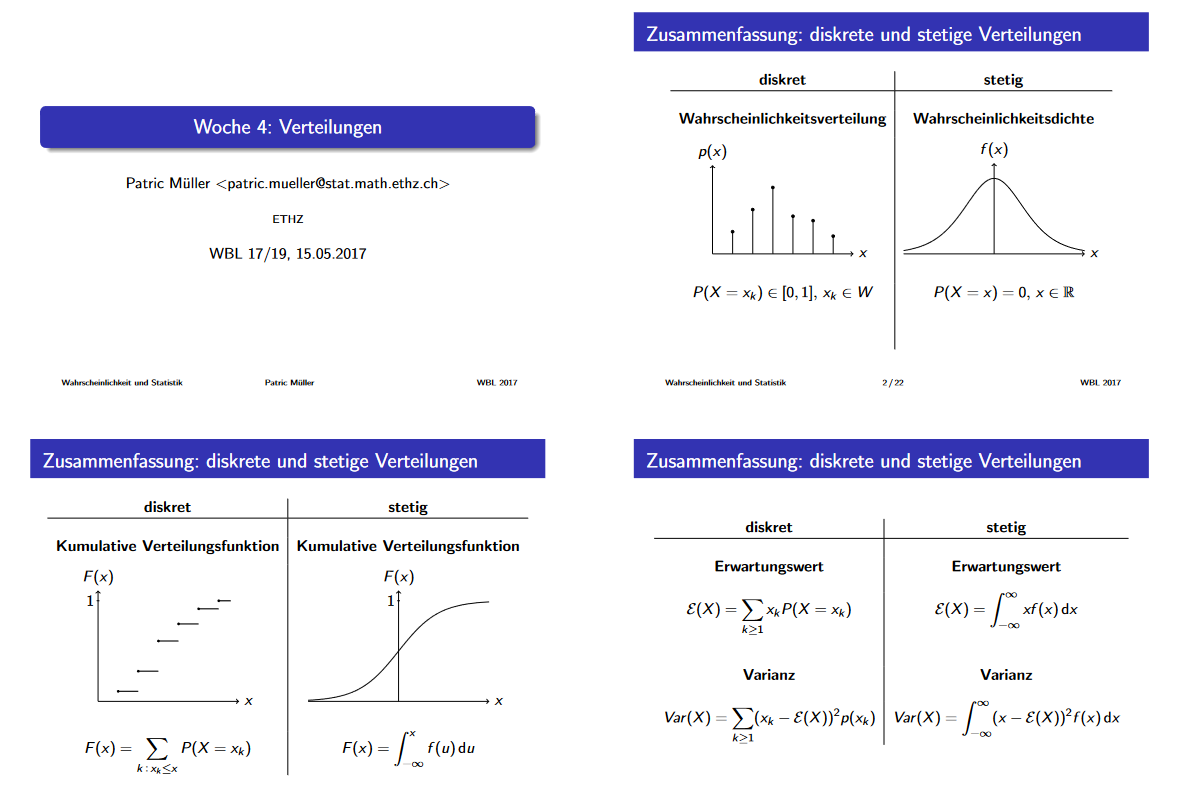
\includegraphics[width=\columnwidth]{diskrete_stetige_verteilung.png}\\
Sein $ (\Omega, \F, P)$ ein Wahrscheinlichkeitsraum. Also $\Omega$ ein
Grundraum, $\F \subseteq 2^\Omega$ die beobachtbaren Ereignisse und $P$ ein
Wahrscheinlichkeitsmass auf $\F$. Eine (reelwertige) Zufallsvariable auf
$\Omega$ ist eine messbare Funktion $X : \Omega \mapsto \R$. Das bedeutet, dass
die Menge $\{X \leq t\} = \{\omega : X (\omega) \leq t\}$ für jedes $t$ ein
beobachtbares Ereigniss sein muss.
\subsection*{Verteilungsfunktion}
Die Verteilungsfunktion von $X$ ist die Abbildung $F_X : \R \mapsto [0, 1]$:
\begin{align*}
  t \mapsto F_X (t) := P[X \leq t] := P[\{\omega : X (\omega) \leq t\}]
\end{align*}
und hat die Eigenschaften:
\begin{itemize}
  \item $F_X$ ist wachsend und rechtsstetig. Das bedeutet,
        dass $F_X (s) \leq F_X (t)$ für $s \leq t$ gilt und $F_X (u) \ra F_X (t)$
        für $u \ra t$ mit $u > t$
  \item $\lim_{t \ra - \infty} F_X (t) = 0$ und $\lim_{t \ra + \infty} F_X (t) = 1$
\end{itemize}
\BoxStart{}
\subsection*{Beispiel: Verteilungsfunktion}
Um zu verhindern, dass ein Gerät infolge eines defekten Halbleiters längere Zeit ausfällt, 
werden zwei identische, parallel geschaltete Halbleiter zu einem Bauteil zusammengefasst.
Eine Kontrolllampe leuchtet auf, wenn einer der beiden Halbleiter ausgefallen ist. 
Wir nehmen an, dass die Lebensdauern der Halbleiter unabhängige, exponentialverteilte Zufallsvariablen mit Erwartungswert 60 Tage sind.
Wie ist die Zeit, nach der die Kontrolllampe ufleuchtet, verteilt? \\

Seien \(H_1\) und \(H_2\) die Lebensdauern der entsprechenden Halbleiter. Nach Voraussetzung sind \(H_1\) und \(H_2\) i.i.d. und 
Exp(\(\lambda\))-verteilt mit \(\lambda = \frac{1}{60}\). Sei \(T\) die Zeit, nach der die Kontrolllampe aufleuchtet; 
also ist \(T = \min\{H_1, H_2\}\).
Die Verteilungsfunktion von \(T\) ist gegeben durch

\begin{align*}
  F_T(t)  &= P [T \leq t] = P [\min\{H_1, H_2\} \leq t]\\
          &= 1 - P [\min\{H_1, H_2\} > t] = 1 - P [H_1 > t, H_2 > t]\\
          &= 1 - P [H_1 > t]P [H_2 > t]\\
          &= (1 - \exp(-2\lambda t)) \mathbf{1}_{[0, \infty)}(t)]
\end{align*}

d.h. \(T\) ist wieder exponentialverteilt mit Parameter \(2\lambda = \frac{1}{30}\).

\BoxEnd{}
\subsection*{Dichtefunktion}
Das Analogon der Gewichtsfunktion im Diskreten Fall. Eine Zufallsvariable $X$
mit Verteilungsfunktion $F_X (t) = P[X \leq t]$ heisst (absolut) stetig mit
Dichte (funktion) $f_X : \R \mapsto [0, \infty)$, falls gilt:
\begin{align*}
  F_X (t) = \int_{-\infty}^t f_X (s) \; dx &  & \text{für alle } t \in \R
\end{align*}
und hat die Eigenschaften:
\begin{itemize}
  \item $f_X \geq 0$ und $f_X = 0$ ausserhalb von $\W (X)$.
  \item $\int_{-\infty}^\infty f_X (s) \; ds = 1$;
        das folgt aus $\lim_{t \ra + \infty} F_X (t) = 1$
\end{itemize}
\subsection*{Gleichverteilung}
Die Gleichverteilung auf dem Intervall $[a, b]$ ist ein Modell für die
Zufällige Wahl eines Punktes in $[a, b]$. Die zugehörige Zufallsvariable $X$
hat den Wertebereich $\W (X) = [a, b]$, sowie
\begin{align*}
  f_X (t) & =
  \begin{cases}
    \frac{1}{b-a} & \text{für } a \leq t \leq b \\
    0             & \text{sonst.}
  \end{cases} \\
  F_X (t) & =
  \begin{cases}
    0               & \text{für } t < a           \\
    \frac{t-a}{b-a} & \text{für } a \leq t \leq b \\
    1               & \text{für } t > b.
  \end{cases}
\end{align*}
wir schreiben kurz $X \sim U (a, b)$.
\begin{align*}
  E[X] = \frac{a + b}{2} &  & Var[X] = \frac{{(b - a)}^2}{12}
\end{align*}
\subsection*{Exponentialverteilung}
Die Exponentialverteilung mit Parameter $\lambda > 0$ ist das stetige Analogon
der Geometrischen Verteilung. Die zugehörige Zufallsvariable $X$ hat $\W (X) =
  [0, \infty)$, Dichte und Verteilungsfunktion:
\begin{align*}
  f_X (t) & =
  \begin{cases}
    \lambda \cdot e^{-\lambda t} & \text{für } t \geq 0 \\
    0                            & \text{für }t < 0
  \end{cases} \\
  F_X (t) & =
  \int_{-\infty}^t f_X (s) \; ds =
  \begin{cases}
    1 - e^{-\lambda t} & \text{für } t \geq 0 \\
    0                  & \text{für }t < 0
  \end{cases}
\end{align*}
wir schreiben kurz $X \sim Exp (\lambda)$. Weiter ist
die Funktion Gedächtsnislos, dh. $\cond{X > t + s}{X > s} = P[X > t]$.
\begin{align*}
  E[X] = \frac{1}{\lambda} &  & Var[X] = \frac{1}{\lambda^2}
\end{align*}
\subsection*{Normalverteilung}
Die Normalverteilung hat zwei Parameter: $\mu \in \R$ und $\sigma^2 > 0$. Die
zugehörige Zufallsvariable $X$ hat den Wertebereich $\W (X) = \R$ und die
Dichtefunktion:
\begin{align*}
  f_X (t) = \frac{1}{\sigma \sqrt{2 \pi}} e^{- \frac{{(t - \mu)}^2}{2 \sigma^2}}
   &  & \text{für } t \in \R
\end{align*}
welche symmetrisch um $\mu$ ist. Wir schreiben kurz: $X \sim \Normalverteilt$.
\subsection*{Standard Normalverteilung}
Wichtige Normalverteilung mit $\Standardnormalverteilt$. Weder für die
zugehörige Dichte $\vp (t)$ noch Verteilungsfunktion $\Phi (t)$ gibt es
geschlossene Ausdrücke, aber das Integral
\begin{align*}
  \Phi (t) = \int_{-\infty}^t \vp (s) \; ds =
  \frac{1}{\sqrt{2\pi}} \int_{-\infty}^t e^{-\frac{1}{2} s^2} \; ds
\end{align*}
ist tabelliert. Ist $X \sim \Normalverteilt$, so ist
$\frac{X - \mu}{\sigma} \sim \Standardnormalverteilt$, also:
\begin{align*}
  F_X (t) = P[X \leq t] = P \left[ \frac{X-\mu}{\sigma} \leq \frac{t - \mu}{\sigma} \right] = \Phi \left  ( \frac{t - \mu}{\sigma} \right)
\end{align*}
deshalb genügt es $\Phi$ zu tabellieren.
\begin{align*}
  \Phi (-z) = 1 - \Phi (z)
\end{align*}
\subsection*{Normalapproximation}
Wenn $S_n \sim Bin (n, p)$ dann
\begin{align*}
  S_n \sim_{approx} N (np, np (1-p))
\end{align*}
\subsection*{Erwartungswert}
Ist $X$ stetig mit Dichte $f_X (x)$, so ist der Erwartungswert:
\begin{align*}
  E[X] = \int_{-\infty}^\infty x \cdot f_X (x) \; dx
\end{align*}
sofern das Integral absolut konvergiert. Ist das Integral nicht
absolut konvergent, so existiert der Erwartungswert nicht.
\subsection*{Erwartungswert einer Funktion}
Sei $X$ eine Zufallsvariable und $Y = g (X)$ eine weitere Zufallsvariable. Ist
$X$ stetig mit Dichte $f_X$, so ist
\begin{align*}
  E[Y] = E[g (X)] = \int_{-\infty}^\infty g (x) \cdot f_X (x) \; dx
\end{align*}
\subsection*{Momente \& Absolute Momente}
Sei $X$ eine Zufallsvariable und $p \in \R^+$. Wir definieren:
\begin{itemize}
  \item $p$-te absolute Moment von $X$: $M_p := E[\abs{X}^p]$
  \item falls $M_n < \infty$ für ein $n$, dann ist das $n$-te (rohe) Moment von $X$
        durch $m_n := E[X^n]$ definiert.
  \item Das $n$-te zentralisierte Moment von $X$ ist durch $\mu_n := E[(X - E[X])^n]$
        definiert.
\end{itemize}
Es gilt weiter, dass $M_n < \infty$ für $n \in \N \implies \abs{m_m} \leq M_n$.
\begin{align*}
  M_p                         & = \int_{-\infty}^\infty \abs{x}^p f_X (x) \; dx \\
  m_n                         & = \int_{-\infty}^\infty x^n f_X (x) \; dx       \\
  p \leq q \land M_q < \infty & \implies M_p < \infty
\end{align*}
\subsection*{Gemeinsame Verteilung/Dichte}
Die Gemeinsame Verteilungsfunktion von Zufallsvariablen $\zufallsvariablen$ ist die Abbildung $F: \R^n \mapsto [0, 1]$ mit:
\begin{align*}
  F (x_1, \dots, x_n) & := P[X_1 \leq x_1, \dots, X_n \leq x_n]                                                 \\
                      & = \int_{-\infty}^{x_1} \dots \int_{-\infty}^{x_n} f (t_1, \dots, t_n) \; dt_n \dots t_1
\end{align*}
dann heisst $f (x_1, \dots, x_n)$ die gemeinsame Dichte, welche folgende
Eigenschaften hat:
\begin{itemize}
  \item $f (x_1, \dots, x_n) \geq 0$ und $= 0$ ausserhalb von $\W (\zufallsvariablen)$.
  \item $\int_{-\infty}^\infty \dots \int_{-\infty}^\infty f (t_1, \dots, t_n) \; dt_n \dots t_1 = 1$
  \item $P[ (\zufallsvariablen) \in A] = \int_{ (x_1, \dots, x_n) \in A} f (t_1, \dots, t_n) \; dt_n \dots t_1$ für $A \subseteq \R^n$
\end{itemize}
\subsection*{Randverteilung}
Haben $X, Y$ die Gemeinsame Verteilungsfunktion $F$, so ist die Funktion $F_X:
  \R \mapsto [0, 1]$,
\begin{align*}
  F_X (x) & = P[X \leq x] = P[X \leq x, Y < \infty] = \lim_{y \ra \infty} F (x, y) \\
  f_X (x) & = \int_{-\infty}^\infty f (x, y) \; dy
\end{align*}

Sind $X, Y$ diskrete Zufallsvariablen mit $\W (Y) = \{y_1, y_2, \dots\}$
und gemeinsamer Gewichtsfunktion $p (x, y)$, so ist die Gewichtsfunktion
der Randverteilung von $X$ gegeben durch:
\begin{align*}
  x \mapsto p_X (x) := \sum_{y_i \in \W (X)} P[X = x, Y = y_i]
\end{align*}
\BoxStart{}
\subsection*{Beispiel: Dichtefunktion berechnen}
Seien $X$ und $Y$ zwei unabhängige Zufallsvariablen, beide exponentialverteilt mit
Parameter $\lambda > 0$. Definiere
\[
  U := \frac{X}{X + Y} und V := X + Y
\]
Seien $f_U$ und $f_V$ die zu $U$ und $V$ gehörigen Dichtefunktionen. Berechne
die Dichtefunktion $f_U$ und Verteilungsfunktion $F_U$
\begin{align*} 
  P[U \leq u] &= \lambda^2 \int_0^\infty e^{-\lambda x} \left(\int_0^\infty 1_{\frac{x}{x + y}\leq u}e^{-\lambda y}dy\right)dx\\ 
  &= \lambda^2 \int_0^\infty e^{-\lambda x} \left(\int_0^\infty 1_{x(u^{-1} - 1)\leq y}e^{-\lambda y}dy\right)dx\\ 
  &= \lambda \int_0^\infty e^{-\lambda x} \left(\int_{x(u^{-1} -1)}^\infty \lambda e^{-\lambda y}dy\right)dx\\ 
  &= \lambda \int_0^\infty e^{-\lambda x} e^{-\lambda x (u^{-1} -1)}dx\\ 
  &= \lambda \int_0^\infty e^{-\lambda u^-1 x}dx\\ 
  &= u 
\end{align*}

\BoxEnd{}
\BoxStart{}
\subsection*{Beispiel: Randverteilung, gemeinsame Dichte}
Man wählt zufällig einen Punkt $P = (U, V)$ in dem Gebiet $D$. Die gemeinsame Dichte von $(U, V)$
\[
  f_{U, V} (u, v) =
  \begin{cases}
    c & \text{falls } (u, v) \in D \\
    0 & \text{sonst}               \\
  \end{cases}
\]
\begin{center}
  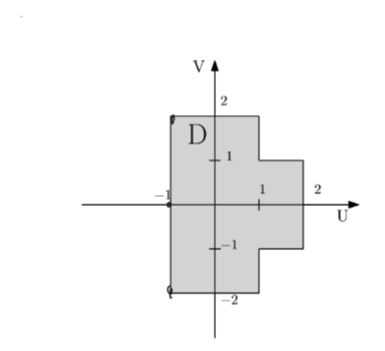
\includegraphics[width=0.2\textwidth]{dichte_aufgabe.png}
\end{center}
\begin{itemize}[noitemsep,topsep=0pt,parsep=0pt,partopsep=0pt]  \item bestimme Konstnte $c$
  \item bestimme Randverteiungsfunktion von U und Randdichtefunktion $f_U(u)$.
  \item Sind $U$ und $V$ unabhängig?
\end{itemize}

\begin{align*}
  D =  & \{(a, b) \in \mathbb{R}^2 : -1 \leq a \leq 1 \text{ and } -2 \leq b \leq 2\} \\
  \cup & \{(a, b) \in \mathbb{R}^2 : 1 \leq a \leq 2 \text{ and } -1 \leq b \leq 1\}  \\
       & f_{U,V}(u, v) =
  \begin{cases}
    1/10 & \text{if } (u, v) \in D \\
    0    & \text{otherwise}
  \end{cases}
\end{align*}
For $u < -1$, $F_U(u) = P(U \leq u) = 0$.
For $-1 \leq u \leq 1$, $F_U(u) = P(U \leq u) = $
\[
  \int_u^{-1} \int_{-2}^{2} \frac{1}{10} \mathbf{1}_D(u, v) \, dv \, ds = \frac{4(u + 1)}{10}
\]

For $1 \leq u \leq 2$, $F_U(u) = P(U \leq u) =$
\[
  \int_1^{-1} \int_{-2}^{2} \frac{1}{10} \mathbf{1}_D(u, v) \, dv \, ds + \int_u^1 \int_{-1}^{1} \frac{1}{10} \mathbf{1}_D(u, v) \, dv \, ds
\]
\[
  = \frac{8}{10} + \frac{2(u - 1)}{10}
\]

and $F_U(u) = 1$ for $u > 2$.

\[
  f_U(u) = \begin{cases}
    \frac{4}{10} & \text{if } -1 \leq u \leq 1 \\
    \frac{2}{10} & \text{if } 1 \leq u \leq 2  \\
    0            & \text{otherwise}
  \end{cases}
\]

\[
  f_V(v) = \int_{-\infty}^{\infty} f_{U,V}(u,v) \, du =
\]
\[
  \frac{1}{2}\left(2[v \in [-2,2]] + [v \in [-1,1]]\right)
\]

If U and V are independent, then for all u and v:

\[
  f_U(u) \cdot f_V(v) = f_{U,V}(u,v)
\]

However, we have \(f_{U,V}(2,2) = 0\) and \(f_U(2) \cdot f_V(2) = \frac{1}{5}
\cdot \frac{1}{5} \neq 0\).

Therefore, U and V are not independent.

\BoxEnd{}
\subsection*{Unabhängigkeit}
Die Zufallsvariablen $\zufallsvariablen$ heissen unabhängig, falls gilt
(äquivalent):
\begin{align*}
  F (x_1, \dots, x_n) = F_{X_1} (x_1) \cdot \hdots \cdot F_{X_n} (X_n) \\
  f (x_1, \dots, x_n) = f_{X_1} (x_1) \cdot \hdots \cdot f_{X_n} (X_n)
\end{align*}
für alle $x_1, \dots, x_n$.
\subsection*{Bedingte Verteilungen}
Es gilt:
\begin{align*}
  f_{X_1 \; | \; X_2} (x_1 \; | \; x_2) & = \frac{f_{X_1,  X_2} (x_1,  x_2)}{f_{X_2} (x_2)}              \\
  \cond{Y > t}{Y < a}                   & = \frac{P[t < Y < a]}{P[Y < a]}                                \\
  E[X_1 \; | \; X_2]                    & = \int x_1 \cdot f_{x_1 \; | \; x_2} (x_1 \; | \; x_2) \; dx_1
\end{align*}
\subsection*{Summen von Zufallsvariablen}
Sei $Z = X + Y$ eine Zufallsvariable mit:
\begin{align*}
  F_Z (z) & = P[Z \leq z] = P[X + Y \leq z]                                     \\
          & = \int_{-\infty}^\infty \int_{-\infty}^{z - x} f (x, y )\; dy \, dx \\
  f_Z (z) & = \int_{-\infty}^\infty f (z - y, y) \; dy
\end{align*}
\subsection*{Transformationen}
Sei $X$ eine Zufallsvariable mit Verteilung und Dichte. Sei $g: \R \mapsto \R$
eine messbare Funktion. Betrachte nun $Y = g (X)$, wir suchen Verteilung und
Dichte von $Y$:
\begin{align*}
  F_Y (t) & = P[Y \leq t] = P[g (Y) \leq t] = \int_{A_g} f_X (s) \; ds \\
  A_g     & := \{s \in \R \; | \; g (s) \leq t\}
\end{align*}
Wobei man die Dichte durch ableiten der Verteilung erhält.
\subsection*{Anwendung von Transformationen}
Sei $F$ eine stetige und streng monoton wachsende Verteilungsfunktion mit
Unkehrfunktion $F^{-1}$. Ist $X \sim \mathcal{U} (0, 1)$ und $Y = F^{-1} (X)$,
so hat $Y$ gerade die Verteilungsfunktion $F$:
\begin{align*}
  F_Y (t) & = P[Y \leq t] = P[F^{-1} (X) \leq t] \\
          & = P[X \leq F (t)] = F (t)
\end{align*}
Mit der Substitution
\begin{align*}
  \phi(X) & = Y                                              \\
  X       & = \phi^{-1}(y)                                   \\
  f_Y(y)  & = f_X(\phi^{-1}(y))|\text{det }J_{\phi^{-1}}(y)| \\
\end{align*}
\BoxStart{}
\subsection*{Beispiel: Transformation}
Sei $X$ eine Zufallsvariable mit Dichte $f_X(x), x \in \R$ und sei $Y = e^X$. Was ist die Dichte $f_Y(y), y > 0$ der Zufallsvariable $Y$?
\begin{align*}
  Y             & = e^X                          \\
  X             & = \ln Y                        \\
  \frac{dx}{dy} & = \frac{1}{y}                  \\
  f_Y(y)        & = f_X(\ln y) \cdot \frac{1}{y} \\
\end{align*}
\BoxEnd{}

\subsection*{Markov Ungleichung}
Sei $X$ eine Zufallsvariable und ferner $g : \W (X) \mapsto [0, \infty)$ eine
wachsende Funktion. Für jedes $c \in \R$ mit $g (c) > 0$ git dann:
\begin{align*}
  P[X \geq c] \leq \frac{E[g (X)]}{g (c)}
\end{align*}
\subsection*{Chebyshev-Ungleichung}
Sei $Y$ eine Zufallsvariable mit endlicher Varianz. Für jedes $b > 0$ git dann:
\begin{align*}
  P[\abs{Y - E[Y]} \geq b] \leq \frac{Var[Y]}{b^2}
\end{align*}
\subsection*{Momenterzeugende Funktion}
Die Momenterzeugende Funktion einer Zufallsvariable $X$ ist:
\begin{align*}
  M_X (t) := E[e^{t \cdot X}] &  & \text{für } t \in \R
\end{align*}

\BoxStart{}
\subsection*{Beispiel: momenterzeugende Funktion}
Sei \(X\) eine exponentialverteilte Zufallsvariable mit Parameter \(\lambda\), d.h. \(X \sim \text{Exp}(\lambda)\). Berechnen Sie die momenterzeugende Funktion \(M_X(t)\).

\begin{align*}
  M_X(t) &= E[e^{tX}] \\
         &= \int_{0}^{\infty} e^{tx} \lambda e^{-\lambda x} \, dx \\
         &= \lambda \int_{0}^{\infty} e^{-(\lambda - t)x} \, dx = -\frac{\lambda}{\lambda - t} e^{-(\lambda - t)x} \bigg|_{0}^{\infty} \\
         &\begin{aligned}
           &= \begin{cases}
                \frac{\lambda}{\lambda - t}, & \text{falls } t < \lambda, \\
                \infty, & \text{falls } t \geq \lambda.
              \end{cases}
           \end{aligned}
\end{align*}
\BoxEnd{}

\subsection*{Grosse Summenabweichung}
Seien $\zufallsvariablen$ i.i.d. Zufallsvariablen, für welche die
Momenterzeugende Funktion $M_X (t)$ für alle $t \in \R$ endlich ist. Für jedes
$b \in \R$ gilt dann:
\begin{align*}
  P[S_n \geq b] \leq \exp \left( \inf_{t \in \R}  ( n \cdot \log M_X (t) - t \cdot b ) \right)
\end{align*}

\subsection*{Chernoff Schranken}
Seien $\zufallsvariablen$ unabhängig mit $X_i \sim Be (p)$ und $X = \Sn X_i$.
Sei $\mu_n := E[X] = \Sn p_i$ und $\delta > 0$. Dann gilt:
Suppose $0 < \delta$, then
\[ P(X \geq (1 + \delta)\mu) \leq e^{-\frac{\delta^2\mu}{2+\delta}}, \]
and
\[ P(X \leq (1 - \delta)\mu) \leq e^{-\frac{\delta^2\mu}{2}}. \]

\BoxStart{}
\subsection*{Beispiel: Chernoff Schranke}
Suppose you toss a fair coin 200 times. How likely is it that you see
at least 120 heads?
The Chernoff bound says

\begin{align*}
  P(X \geq 120) &= P(X \geq (1 + \frac{20}{100}) \cdot 100) \leq e^{-\frac{1}{5^2} \cdot \frac{100}{2+\frac{1}{5}} \cdot 100} \\
                &= e^{-\frac{20}{6}} = 0.0356
\end{align*}

\BoxEnd{}
\subsection*{Schwaches Gesetz der grossen Zahlen}
Sei $X_1, X_2, \dots$ eine Folge von unabhängigen Zufallsvariablen, die alle
den gleichen Erwartungswert $E[X_i] = \mu$ und die gleiche Varianz $Var[X_i] =
  \sigma^2$ haben. Sei
\begin{align*}
  \overline{X}_n = \frac{1}{n} S_n = \frac{1}{n} \Sn X_i
\end{align*}
Dann konvergiert $\overline{X}_n$ für $n \ra \infty$ in Wahrscheinlichkeit/
stochastisch gegen $\mu = E[X_i]$, d.h.:
\begin{align*}
  P \left[ \abs{\overline{X}_n - \mu} > \varepsilon \right] \underset{n \ra \infty}{\longrightarrow} 0
   &  & \text{für jedes } \varepsilon > 0
\end{align*}
(Statt unabhängig genügt auch $Cov (X_i, X_k) = 0$ für $i \neq k$)
\subsection*{Starkes Gesetz der grossen Zahlen}
Sei $X_1, X_2, \dots$ eine Folge von unabhängigen Zufallsvariablen, die alle
dieselbe Verteilung haben, und ihr Erwartungswert $\mu = E[X_i]$ sei endlich.
Für:
\begin{align*}
  \overline{X}_n = \frac{1}{n} S_n = \frac{1}{n} \Sn X_i
\end{align*}
gilt dann
\begin{align*}
  \overline{X}_n \underset{n \ra \infty}{\longrightarrow} \mu &  & \text{P-fastsicher}
\end{align*}
d.h.:
\begin{align*}
  P \left[ \left\{ \omega \in \Omega : \overline{X}_n (\omega) \underset{n \ra \infty}{\longrightarrow} \mu \right\} \right] = 1
\end{align*}
\subsection*{i.i.d. / u.i.v.}
Independent identically distributed
\subsection*{Zentraler Grenzwertsatz}
Sei $X_1, X_2, \dots$ eine Folge von i.i.d. Zufallsvariablen mit $E[X_i] = \mu$
und $Var[X_i] = \sigma^2$. Für die Summe $S_n = \Sn X_i$ gilt dann:
\begin{align*}
  \lim_{n \ra \infty} P \left[ \frac{S_n - n \cdot \mu}{\sigma \sqrt{n}} \leq x \right] = \Phi (x)
   &  & \text{für alle } x \in \R
\end{align*}
wobei $\Phi$ die Verteilungsfunktion von $\Standardnormalverteilt$ ist.
{\section{Statistik}}
\subsection*{$\X^2$-Verteilung}
Die $\X^2$- Verteilung mit $n$ Freiheitsgraden (bez. $\X^2_n$) gehört zu einer
stetigen Zufallsvariable $Y$ mit Dichtefunktion:
\begin{align*}
  f_Y (y) = \frac{1}{2^{\frac{n}{2}}  \Gamma (\frac{n}{2})} y^{\frac{n}{2} - 1} e^{-\frac{1}{2} y}
\end{align*}
wobei dies ein Spezialfall der $Ga (\alpha, \lambda)$ Verteilung ist mit
$\alpha = \frac{n}{2}$ und $\lambda = \frac{1}{2}$. Sind die Zufallsvariablen
$\zufallsvariablen$ i.i.d. $\sim \Standardnormalverteilt$, so ist die Summe
$Y := \Sn X_i^2 \sim \X^2_n$.
\subsection*{$t$-Verteilung}
Die $t$-Verteilung mit $n$ Freiheitsgraden gehört zu einer stetigen
Zufallsvariable $Z$ mit Dichtefunktion
\begin{align*}
  f_Z (z) = \frac{\Gamma (\frac{n+1}{2})}{\sqrt{n \pi} \, \Gamma (\frac{n}{2})} \left( 1 + \frac{z^2}{n} \right)^{-\frac{n+1}{2}}
   &  & \text{für } z \in \R
\end{align*}
für $n = 1$ ist das eine Cauchy Verteilung und für $n \ra \infty$ erhält man
$\Standardnormalverteilt$. Sind $X, Y$ unabhängig und $X \sim \Standardnormalverteilt$
und $Y \sim \X^2_n$, so ist der Quotient:
\begin{align*}
  Z := \frac{X}{\sqrt{\frac{1}{n} Y}} \sim t_n \text{, also $t$-Verteilt mit $n$ Freiheitsgraden}
\end{align*}
\subsection*{Hypothesen}
Es gibt:
\begin{itemize}
  \item Hypothese $H_0 : \vt \in \varTheta_0$
  \item Alternative $H_A : \vt \in \varTheta_A$
\end{itemize}
Man verwirft die Hypothese genau dann, wenn der realisierte Wert im
Verwerfungsbereich $K$ liegt.
\subsection*{Fehler}
Es gibt folgende Fehler:
\begin{itemize}
  \item 1. Art: Hypothese wird zu unrecht abgelehnt. $P_\vt[T \in K]$ für $\vt \in \varTheta_0$
  \item 2. Art: Hypothese wird zu unrecht nicht verworfen. $P_\vt[T \not \in K]$ für $\vt \in \varTheta_A$
\end{itemize}


Meisst kann man nicht beides minimieren, also geht man wie folgt vor:
\begin{enumerate}
  \item Man wählt ein \textbf{Signifikanzniveau} $\alpha \in (0, 1)$ und kontrolliert
        die Wahrscheinlichkeit eines Fehlers 1. Art durch
        \begin{align*}
          \sup_{\vt \in \varTheta_0} P_\vt[T \in K] \leq \alpha
        \end{align*}
  \item Man versucht die Wahrscheinlichkeit für einen Fehler zweiter Art $P_\vt[T \not
            \in K]$ für $\vt \in \varTheta_A$ zu minimieren. Dazu maximiert man die
        \textbf{Macht des Tests}:
        \begin{align*}
          \beta : \varTheta_A \mapsto [0, 1] &  & \vt \mapsto \beta (\vt) := P_\vt[T \in K]
        \end{align*}
\end{enumerate}
Somit ist es schwieriger eine Hypothese zu verwerfen als zu behalten. In einem
Test \textbf{verwendet man deshalb immer als Hypothese die Negation der eigentlich gewünschten Aussage.}
\BoxStart{}
\subsection*{Beispiel: Was passiert, wenn das Signifikanzniveau $\alpha$ kleiner wird?}
Kleineres Signifikanzniveau ($\alpha$)
\begin{itemize}
  \item Engerer Verwerfungsbereich
  \item Weniger extreme Teststatistikwerte für Ablehnung der Nullhypothese erforderlich
  \item Strengerer Test
  \item Höhere Anforderungen an statistische Signifikanz
  \item Geringere Wahrscheinlichkeit, Nullhypothese fälschlicherweise abzulehnen
  \item Höhere Wahrscheinlichkeit für Fehler vom Typ II (falsche Akzeptanz der Nullhypothese, wenn sie in Wirklichkeit falsch ist)
  \item Macht wird reduziert
\end{itemize}
\BoxEnd{}

\BoxStart{}
\subsection*{Beispiel: Hypothesen-Test}
Wir haben eine Münze mit einer Seite rot und der anderen Seite
blau gefärbt, und wir vermuten, dass die Münze gezinkt ist und eher auf der
blauen Seite landet.
\begin{enumerate}[leftmargin=0.4cm]
  \item \textbf{Modell:} Unter $P_p$ sind die $X_i$ i.i.d., $\sim Ber(p), i = 1, \ldots, 10, p$ unbekannt
  \item \textbf{Nullhypothese: }$H_0 : p = p_0 = 0.5$
  \item \textbf{Alternativhypothese: } \(H_A: p = p_A > p_0\).
  \item \textbf{Teststatistik: } \(T = \sum_{i=1}^{10} X_i\), denn
  \begin{align*}
    &R(x_1, \ldots , x_{10}; \lambda_0, \lambda_A) \\
    &= L(x_1, \ldots , x_{10}; \lambda_0) L(x_1, \ldots , x_{10}; \lambda_A)\\ 
    &= \frac{p_0^T (1 - p_0)^{10-T}}{p_A^T (1 - p_A)^{10-T}}\\
    &= \left(\frac{p_0(1 - p_A)}{p_A(1 - p_0)}\right)^T \left(\frac{1 - p_0}{1 - p_A}\right)^{10}
  \end{align*}
  Da \(\frac{p_0(1-p_A)}{p_A(1-p_0)} < 1\) wird \(R(x_1, \ldots , x_{10}; p_0, p_A)\) klein, genau dann, wenn \(\sum_{i=1}^{10} x_i\) groß ist. Wir wählen als Teststatistik also \(T = \sum_{i=1}^{10} X_i\).
  \item \textbf{Verteilung der Teststatistik unter \(H_0\): } \(T \sim \text{Bin}(10, 1/2)\).
  \item \textbf{Verwerfungsbereich: } Der kritische Bereich "Quotient klein" hat die äquivalente Form "Summe groß", also ist der Verwerfungsbereich von der Form \(K = (k, \infty)\). Um das Signifikanzniveau einzuhalten, muss gelten
  \[ P_{p_0}[T \in K] = P_{p_0}[T > k] \leq 1\% \Rightarrow P_{p_0}[T \leq k] \geq 99\%. \]
  Deshalb haben wir als Verwerfungsbereich \(K = (9, \infty)\).
  \item \textbf{Beobachteter Wert der Testst.: } \(t = T(\omega) = 8\).
  \item \textbf{Testentscheid: } Da 8 nicht im Verwerfungsbereich liegt, wird die Nullhypothese nicht verworfen.
    

\end{enumerate}
\BoxEnd{}
\subsection*{Hypothesis testing}
\begin{enumerate}
  \item \textbf{Left-sided or left-tailed test: } If $H_0 : p = p_0$ is tested against the alternative $H_1 : p < p_0$, the region of rejection has the form $\{0, 1, \ldots, k\}$. The critical value $k$ is the largest value such that $P(X \leq k) \leq \alpha$.
  \item \textbf{Right-sided or right-tailed test: } If \(H_0 : p = p_0\) is tested against the alternative \(H_1 : p > p_0\), the region of rejection has the form \(\{k, k + 1, \ldots , n\}\). The critical value \(k\) is the smallest value such that \(P(X \geq k) \leq \alpha\).
  \item \textbf{Two-sided or two-tailed test: } If \(H_0 : p = p_0\) is tested against the alternative \(H_1 : p \neq p_0\), the region of rejection has the form \(K = \{0, 1, \ldots , k_1\} \cup \{k_2, k_2+1, \ldots , n\}\). The critical values \(k_1\) and \(k_2\) are determined as the smallest and largest value, respectively, such that \(P(X \leq k_1) \leq \frac{\alpha}{2}\) and \(P(X \geq k_2) \leq \frac{\alpha}{2}\).

\end{enumerate}

\subsection*{Likelihood Quotient}
Sei $L (x_1, \dots, x_n; \vt)$ die Likelihood Funktion und $\vt_0 \in
  \varTheta_0$ sowie $\vt_A \in \varTheta_A$. Dann definieren wir:
\begin{align*}
  R (x_1, \dots, x_n; \vt_0, \vt_A) = \frac{L (x_1, \dots, x_n; \vt_A)}{L (x_1, \dots, x_n; \vt_0)}
\end{align*}
je grösser der Quotient, desto wahrscheinlicher die Alternative. Es gibt auch:
\begin{align*}
  R (x_1, \dots, x_n)             & = \frac{ \sup_{\vt \in \varTheta_A} L (x_1, \dots, x_n; \vt)}{\sup_{\vt \in \varTheta_0} L (x_1, \dots, x_n; \vt)}                  \\
  \widetilde{R} (x_1, \dots, x_n) & = \frac{ \sup_{\vt \in \varTheta_A \cup \varTheta_0} L (x_1, \dots, x_n; \vt)}{\sup_{\vt \in \varTheta_0} L (x_1, \dots, x_n; \vt)} \\
\end{align*}
Wähle Konstante $c_0$ für $K_0 =  (c_0, \infty)$ mithilfe von Signifikanzniveau.
\subsection*{Neyman-Pearson Lemma}
Sei $\varTheta_0 = \{\vt_0\}$ und $\varTheta_A = \{\vt_A\}$. Wie oben sei $T =
  R (\zufallsvariablen; \vt_0, \vt_A)$ und $K := (c, \infty)$, sowie $\alpha^* :=
  P_{\vt_0}[T \in K] = P_{\vt_0}[T > c]$. Der Likelihood Quotienten Test mit
Teststatistik $T$ und kritischem Bereich $K$ ist dann in folgendem Sinn
optimal: Jeder andere Test mit Signifikanzniveau $\alpha \leq \alpha^*$ hat
eine kleinere Macht (bez. Grössere WS Fehler 2. Art).
\subsection*{$p$-Wert}
(Nach Wikipedia) Der $p$-Wert ist die Wahrscheinlichkeit ein mindestens
so extremes Testergebnis zu erhalten, wenn die Nullhypothese gelten würde:
\begin{align*}
  p (x) & = \cond{X \leq x}{H_0} \text{   oder   } \cond{X \geq x}{H_0}   \\
  p (x) & = 2 \cdot \min \{ \cond{X \leq x}{H_0}, \cond{X \geq x}{H_0} \}
\end{align*}
\subsection*{$z$-Test}
Normalverteilung, Test für Erwartungswert bei bekannter Varianz. Hier sind
$\zufallsvariablen$ i.i.d. $\mathcal{N} (\vt, \sigma^2)$. Wir möchten die
Hypothese $H_0 : \vt = \vt_0$ testen. Mögliche Alternativen $H_A$ sind $\vt >
  \vt_0$, $\vt < \vt_0$ (einseitig) oder $\vt \neq \vt_0$ (zweiseitig). Die
Teststatistik ist:
\begin{align*}
  T & = \frac{\overline{X} - \vt_0}{\sigma / \sqrt{n}} \sim \Standardnormalverteilt
    &                                                                               & \text{unter } P_{\vt_0}
\end{align*}
Und die Verwerfungsbereich:
\begin{align*}
  \vt < \vt_0    &  & (-\infty, z_\alpha)                                                      \\
  \vt > \vt_0    &  & (z_{1 - \alpha}, \infty)                                                 \\
  \vt \neq \vt_0 &  & (-\infty, z_{\frac{\alpha}{2}}) \cup  (z_{1 - \frac{\alpha}{2}}, \infty)
\end{align*}
Wobei die $z$ Werte in der Tabelle nachgeschaut werden können
und es gilt $z_\alpha = - z_{1 - \alpha}$.

\BoxStart{}
\subsection*{Beispiel Fehler 1. Art berechnen}
Sei $\Theta = [0, 1]$ und seien $X_1, \ldots , X_6$ unabhängig, identisch verteilt unter $P_\theta$
mit $X_i \sim \text{Ber}(\theta)$. Wir betrachten die Nullhypothese $H_0 : \theta = \frac{1}{2}$ und die Alternativhypothese
$H_A : \theta = \frac{1}{3}$. Wie hoch ist die Wahrscheinlichkeit eines Fehlers 1. Art für den Test $(T, K)$ mit
$T = \sum_{i=1}^{6} X_i$ und $K = (-\infty, 0]$?

Die Teststatistik $T$ ist die Summe der beobachteten Werte der $X_i$:
\begin{align*}
  P(T \in K)  &= P[T \leq 0] = P[T = 0] \\
              &= P(X_1 = 0) \cdot P(X_2 = 0) \cdot \ldots \cdot P(X_6 = 0)\\
              &= \left( \frac{1}{2} \right)^6 = \frac{1}{64} 
\end{align*}



\BoxEnd{}
\BoxStart{}
\subsection*{Beispiel Fehler 2. Art berechnen}
Nehme an: einseitiger $z$-Test, $T = \frac{\overline{X}_n - \mu_0}{\sigma /
    \sqrt{n}}$, $\mu_0 = 70$.
\begin{align*}
  H_0 : \mu = \mu_0 &  & H_A : \mu < \mu_0
\end{align*}
Kritischer Bereich mit $5$\% niveau: $K =  (- \infty, -1.645)$. Wir
nehmen an, dass $T = \frac{\overline{X}_n - \mu_A}{\sigma / \sqrt{n}} \sim \Standardnormalverteilt$:
\begin{align*}
  P_{\mu_A}[T \not \in K]
   & = P_{\mu_A}[T > -1.645]                                                                                                            \\
   & = P_{\mu_A} \left[\frac{\overline{X}_n - \mu_0}{\sigma / \sqrt{n}} > -1.645 \right]                                                \\
   & = P_{\mu_A} \left[\frac{\overline{X}_n - \mu_A}{\sigma / \sqrt{n}} > \frac{\mu_0 - \mu_A}{\sigma / \sqrt{n}} -1.645 \right]        \\
   & = 1 - P_{\mu_A} \left[\frac{\overline{X}_n - \mu_A}{\sigma / \sqrt{n}} \leq \frac{\mu_0 - \mu_A}{\sigma / \sqrt{n}} -1.645 \right] \\
   & = 1 - \Phi \left( \frac{\mu_0 - \mu_A}{\sigma - \sqrt{n}} - 1.645 \right) \\
   & \text{Weil } \sim \Standardnormalverteilt
\end{align*}
\BoxEnd{}
\subsection*{$t$-Test}
Normalverteilung, Test für Erwartungswert bei unbekannter Varianz. Hier sind
$\zufallsvariablen$ i.i.d. $\sim \Normalverteilt$ unter $P_{\vec{\vt}}$, wobei
$\vec{\vt} = (\mu, \sigma^2)$. Wir wollen die Hypothese $\mu = \mu_0$ testen.
Die Teststatistik ist:
\begin{align*}
  T   & := \frac{\overline{X}_n - \mu_0}{S / \sqrt{n}} \sim t_{n-1}
      &                                                             & \text{unter } P_{\vt_0} \\
  S^2 & = \frac{1}{n-1} \Sn  (X_i - \overline{X}_n)^2
\end{align*}
Und die Verwerfungsbereiche:
\begin{align*}
  c_<      & = t_{n-1, \alpha}               &  & (-\infty, c_<)                     &  & \mu < \mu_0    \\
  c_>      & = t_{n-1, 1 - \alpha}           &  & (c_>, \infty)                      &  & \mu > \mu_0    \\
  c_{\neq} & = t_{n-1, 1 - \frac{\alpha}{2}} &  & (-\infty, c_<) \cup  (c_>, \infty) &  & \mu \neq \mu_0
\end{align*}
Wobei gilt $t_{m, \alpha} = -t_{m, 1 - \alpha}$.
\subsection*{Gepaarter Zweiproben-Test}
Hier sind $\zufallsvariablen$ i.i.d. $\sim \mathcal{N} (\mu_X, \sigma^2)$ und
$Y_1, \dots, Y_n$ i.i.d. $\sim \mathcal{N} (\mu_Y, \sigma^2)$ unter $P_\vt$.
Insbesondere ist $m = n$ und die Varianz beider Stichproben dieselbe.
Differenzen $Z_i := X_I - Y_i$ sind unter $P_\vt$ i.i.d. $\mathcal{N} (\mu_X -
  \mu_Y, 2 \sigma^2)$. Dann analog $z$ und $t$-Test. (Setzt natürliche Paarung
von Daten voraus!)
\subsection*{Ungepaarter Zweiproben-Test}
Hier sind unter $P_\vt$ die Zufallsvariablen $\zufallsvariablen$ i.i.d. $\sim
  \mathcal{N} (\mu_X, \sigma^2)$ und $Y_1, \dots, Y_m$ i.i.d. $\sim \mathcal{N}
  (\mu_Y, \sigma^2)$, wobei die Varianz in beiden Fällen dieselbe ist.
\begin{itemize}
  \item Bei bekannter Varianz:
        \begin{align*}
          H_0 & : \mu_X - \mu_Y = \mu_0 \quad  (z.B. \; \mu_0 = 0)                                                                                \\
          T   & = \frac{\overline{X}_n - \overline{Y}_m -  (\mu_X - \mu_Y)}{\sigma \sqrt{\frac{1}{n} + \frac{1}{m}}} \sim \Standardnormalverteilt
        \end{align*}
        Die kritischen Werte für den Verwerfungsbereich sind wie oben
        geeignete Quantile der $\Standardnormalverteilt$-Verteilung, je nach
        Alternative. Das ist der ungepaarte Zweistichproben-$z$-Test.

  \item Bei unbekannter Varianz:
        \begin{align*}
          S_X^2 & := \frac{1}{n-1} \Sn  (X_i - \overline{X}_n)^2                                                                 \\
          S_Y^2 & := \frac{1}{m-1} \sum_{j = 1}^m  (Y_j - \overline{Y}_m)^2                                                      \\
          S^2   & := \frac{1}{m+n-2} \left(  (n-1) \cdot S_X^2 +  (m-1) \cdot S_Y^2 \right)                                      \\
          T     & = \frac{\overline{X}_n - \overline{Y}_m -  (\mu_X - \mu_Y)}{S \sqrt{\frac{1}{n} + \frac{1}{m}}} \sim t_{n+m-2}
        \end{align*}
        unter jedem $P_\vt$. Dieser Test heisst ungepaarter Zweistichproben-$t$-Test.
\end{itemize}
\subsection*{Konfidenzbereich}
Ein Konfidenzbereich für $\vt$ zu Daten $x_1, \dots, x_n$ ist eine Menge $C
  (x_1, \dots, x_n) \subseteq \varTheta$. Damit ist $C (\zufallsvariablen)$ eine
zufällige Teilmenge von $\varTheta$. Dieses $C$ heisst Konfidenzbereich zum
Niveau $1 - \alpha$, falls für alle $\vt \in \varTheta$ gilt:
\begin{align*}
  P_\vt [\vt \in C (\zufallsvariablen)] \geq 1 - \alpha
\end{align*}
\BoxStart{}
\subsection*{Beispiel: Konfidenzbereich}
Machen wir den Ansatz:
\begin{align*}
  C (\zufallsvariablen) = [\overline{X}_n - \dots, \overline{X}_n + \dots]
\end{align*}
so wollen wir erreichen, dass gilt:
\begin{align*}
  1 - \alpha \leq P_\vt[\vt \in  C (\zufallsvariablen)] \\
  = P_\vt \left[ \mu \in [\overline{X}_n - \dots, \overline{X}_n + \dots] \right]
  = P_\vt \left[ \abs{\overline{X}_n - \mu} \leq \dots \right]
\end{align*}
Nach Satz 7.1 ist für jedes $\vt \in \varTheta$:
\begin{align*}
  \frac{\overline{X}_n - \mu}{S / \sqrt{n}} \sim t_{n-1} &  & \text{unter } P_\vt \\
  1 - \alpha \leq P_\vt \left[ \abs{\frac{\overline{X}_n - \mu}{S / \sqrt{n}}} \leq \frac{\dots}{S / \sqrt{n}} \right]
\end{align*}
also erhalten wir das Konfidenzintervall für $\mu$ zum Niveau $1 - \alpha$:
\begin{align*}
  C (\zufallsvariablen) = \left[ \overline{X}_n - t_{n-1, 1 - \frac{\alpha}{2}} \frac{S}{\sqrt{n}}, \overline{X}_n + t_{n-1, 1 - \frac{\alpha}{2}} \frac{S}{\sqrt{n}} \right]
\end{align*}
\BoxEnd{}

% chktex-file 13
% chktex-file 12
% chktex-file 11

{\section{Schätzer}}
\subsection*{Schätzer}
Wir suchen ein Modell für eine Stichprobe $\zufallsvariablen$ und haben einen
Parameteraum $\vartheta \subseteq \varTheta$ und für jedes $\vt$ einen
Wahrscheinlichkeitsraum $ (\Omega, \F, P_\vt)$. Wir möchten nun die Parameter
$\vt_1, \dots, \vt_m$ bestimmen. Ein Schätzer $T_j$ für einen Parameter $\vt_j$
ist eine Zufallsvariable der Form $T_j := t_j (\zufallsvariablen)$ für eine
Schätzfunktion $t_j$.
\subsection*{Schätzwert}
Ein Schätzwert ist das Ergebnis einer konkreten Berechnung, eine Zahl. Sie
entsteht durch das Einsetzen konkreter Daten in einen Schätzer: $T_j (\omega) =
  t_j (x_1, \dots, x_n)$ und liefert damit einen Wert für genau einen Parameter.
\subsection*{Eigenschaften von Schätzern}
Sei $T$ ein Schätzer.
\begin{itemize}
  \item $T$ ist erwartungstreu, falls $E_\vt[T] = \vt$ gilt. $T$ schätzt
        im Mittel also richtig.
  \item Bias $:= E_\vt[T] - \vt$. Ein erwartungstreuer Schätzer hat also keinen Bias.
  \item Mittlere Quadratische Schätzfehler $MSE_\vt[T] := E_\vt[ {(T - \vt)}^2]$.
  \item Eine Folge $T^{ (n)}$ von Schätzern heisst konsistent für $\vt$, falls $T^{
              (n)}$ für $n \ra \infty$ in $P_\vt$-Wahrscheinlichkeit gegen $\vt$ konvergiert,
        d.h. für jedes $\vt \in \varTheta$ gilt:
        \begin{align*}
          \lim_{n \ra \infty} P_\vt \left[ \abs{T^{ (n)} - \vt} > \varepsilon \right] = 0
        \end{align*}
\end{itemize}
\BoxStart{}
\subsection*{Beispiel: Erwartungstreuer Schätzer}
Seien $X_1, \ldots, X_n$ unabhängige, identisch verteilte Zufallsvariablen mit $X_i \sim \mathcal{U}([\theta - 1, \theta]) unter \mathbb{P}_\theta$ 
wobei $\theta \in \mathbb{R}$. Wir betrachten den Schätzer 
\[T_1^{(n)} := \frac{1}{n} \cdot \sum_{i = 1}^n X_i + \frac{1}{2}\]
Sind Schätzer erwartungstreu?

Sei $\theta \in \mathbb{R}$ fixiert. Aus der Gleichverteilung folgt, dass

\begin{align*}
  \mathbb{E}_{\theta}[{T(n)}_1] &= \left(\frac{1}{n} \sum_{i=1}^{n} \mathbb{E}_{\theta}[X_i]\right) + \frac{1}{2} \\
                                &= \mathbb{E}_{\theta}[X_1] + \frac{1}{2} = \theta - \frac{1}{2} + \frac{1}{2} \\
                                &= \theta
\end{align*}
Somit folgt, dass der Schätzer ${T(n)}_1$ erwartungstreu ist.

\BoxEnd{}
\subsection*{Maximum-Likelihood Methode}
(Analog im diskreten Fall.) In einem Modell $P_\vt$ sind die Zufallsvariablen
$\zufallsvariablen$ stetig mit einer gemeinsamen Dichtefunktion
$f (x_1, \dots, x_n, \vt)$. Oft sind die $X_i$ i.i.d. und man erhält:
\begin{align*}
  f (x_1, \dots, x_n, \vt) & = P[X_1 = x_1, \dots, X_n = x_n] \\
                           & = \prod_{i = 1}^n f_X (x_i, \vt)
\end{align*}
Wir nehmen nun an, dass die Daten die wir erhalten haben sehr
Wahrscheinlich sind und versuchen nun folgende Likelihood funktion
zu Maximieren durch Anpassungen an $\vt$:
\begin{align*}
  L (x_1, \dots, x_n; \vt)      & := f (x_1, \dots, x_n; \vt)      \\
  \log L (x_1, \dots, x_n; \vt) & := \log f (x_1, \dots, x_n; \vt)
\end{align*}
letzteres kann bei Produkt zu Summe umwandlung hilfreich sein.
\BoxStart{}
\subsection*{Beispiel: Maximum Likelyhood-Funktion}
Sei $\Theta = [0, 1]$. Wir betrachten die Modellfamilie $ {P_\theta}_{\theta \in \Theta}$, wobei $X_1, \ldots, X_n$ unter $\mathbb{P}_\theta$ unabhängig und identisch verteilt sind mit $X_1 \sim \text{Geom} (\theta)$. Was ist die Likelihood-Funktion $L (x_1, \ldots, x_n; \theta)$ für $x_1, \ldots, x_n \in \{1, 2, \ldots\}$?
\begin{align*}
  L (x_1, \ldots, x_n; \theta) & =  (P_\theta) [X_1 = x_1,\ldots , X_n = x_n]            \\
                               & =\prod_{i = 1}^n \mathbb{P}_\theta[X_i = x_i]           \\
                               & = \theta^n \cdot  {(1 - \theta)}^{x_1 + \ldots + x_n - n}
\end{align*}
\\
Was ist der Maximum-Likelihood-Schätzer $T_{\text{ML}}$ für $\theta$?

\[
  n \cdot \log (\theta) +  (x_1 + \ldots + x_n - n) \cdot \log (1 - \theta)
\]

Wir setzen nun die Ableitung der log-Likelihood-Funktion nach $\theta$ gleich
$0$ und erhalten:

\begin{align*}
   & \frac{n}{\theta} - \frac{x_1 + \ldots + x_n - n}{1 - \theta} = 0               \\
   & \Longleftrightarrow n - n\theta =  (x_1 + \ldots + x_n) \cdot \theta - n\theta \\
   & \Longleftrightarrow \theta = \frac{n}{x_1 + \ldots + x_n}                      \\
   & = \frac{n}{X_1 + \ldots + X_n}
\end{align*}

\BoxEnd{}
\subsection*{Empirisches Moment}
Für $k \in \{1, \dots, m\}$ sei das $k$-te Moment empirische Moment oder
Stichprobenmoment $\hat{m}_k$ der Realisierung $ (x_1, \dots, x_n)$:
\begin{align*}
  \hat{m}_k (x_1, \dots, x_n) := \frac{1}{n} \Sn x_i^k
\end{align*}
\subsection*{Momentenmethode}
Der Momentenmethode liegt zugrunde, dass die Momente einer Zufallsvariable bzw.
einer Wahrscheinlichkeitsverteilung durch Stichprobenmomente geschätzt werden
können.\\ Sei $\zufallsvariablen$ eine Stichprobe und $\varTheta$ der
Parameterraum. Für jeden Parameter $\vt = (\vt_1, \dots, \vt_m) \in \varTheta$
sei $\zufallsvariablen$ i.i.d. unter dem Wahrscheinlichkeitsraum $ (\Omega, \F,
  P_\vt)$. Methode:
\begin{enumerate}
  \item Für gegebene Realisierungen $x_1, \dots, x_n$ bestimme für jedes $k \in \{1,
          \dots, m\}$ das $k$-te empirische Moment
  \item Stelle ein Gleichungssystem für die Unbekannten Parameter $\vt_1, \dots, \vt_m$
        auf, in dem das $k$-te empirische Moment dem $k$-ten Moment gleichgesetzt wird,
        also:
        \begin{align*}
          \hat{m}_k (x_1, \dots, x_n) = g_k (\vt_1, \dots, \vt_m)
           &  & k \in \{1, \dots, m\}
        \end{align*}
  \item Existiert eine Eindeutige Lösung so wird das unsere Schätzung für $\vt$.
\end{enumerate}
\subsection*{Momentenschätzer}
Der Vektor $\hat{\vt} (X_1, \dots, X_m)$ heisst Momentenschätzer des Parameters
$\vt$.
\BoxStart{}
\subsection*{Beispiel: Normalverteile Stichprobe}
Sei $\zufallsvariablen$ i.i.d. $\Normalverteilt$-verteilt mit unbekannten
Parametern $\vt = (\mu, \sigma^2)$. Damit berechnen wir mit der $\log$ max
likelihood funktion Ableitungen setzen diese zu $0$ und bekommen:
\begin{align*}
  T_1 & = \frac{1}{n} \Sn X_i = \overline{X}_n     \\
  T_2 & = \frac{1}{n} \Sn {X_1 - \overline{X}_n}^2
\end{align*}
möchten wir aber noch, dass der Schätzer erwartungstreu wird,
so wählen wir für $T_2 = S^2$:
\begin{align*}
  S^2 = \frac{1}{n-1} \Sn  {(X_i - \overline{X}_n)}^2
\end{align*}
\BoxEnd{}
\subsection*{Normalverteile Stichproben}
Seien $\zufallsvariablen$ i.i.d. $\sim \Normalverteilt$. Dann gilt:
\begin{itemize}
  \item $\overline{X}_n \sim \mathcal{N} (\mu, \frac{\sigma^2}{n})$
        und $\frac{\overline{X}_n - \mu}{\sigma / \sqrt{n}} \sim \Standardnormalverteilt$.
  \item $\frac{n-1}{\sigma^2} S^2 = \left( \frac{1}{\sigma^2} \Sn  {(X_i - \overline{X}_n)}^2 \right) \sim \mathcal{X}^2_{n-1}$
  \item $\overline{X}_n$ und $S^2$ sind unabhängig
  \item $\frac{\overline{X}_n - \mu}{S / \sqrt{n}} = \frac{ \frac{\overline{X}_n - \mu}{\sigma / \sqrt{n}} }{S / \sigma} = \frac{ \frac{\overline{X}_n - \mu}{\sigma / \sqrt{n}} }{\sqrt{\frac{1}{n-1} \frac{n-1}{\sigma^2} S^2}} \sim t_{n-1}$
\end{itemize}

\input{Kapitel8}

\section{Tabellen}
\subsection*{Ableitung, Integration}
Es gilt:
\begin{itemize}
  \item \textbf{Summenregel} $ (f (x) + g (x))' = f' (x) + g' (x)$
  \item \textbf{Produktregel} $ (f (x) \cdot g (x))' = f' (x) \cdot g (x) + f (x) \cdot g' (x)$
  \item \textbf{Quotientenregel} $\left( \frac{f (x)}{g (x)} \right)' = \frac{f' (x) \cdot g (x) - f (x) \cdot g' (x)}{g^2 (x)}$ wenn $g (x) \neq 0$
  \item \textbf{Kettenregel} $ (f (g (x)))' = f' (g (x)) \cdot g' (x)$
  \item \textbf{Partielle Integration} $\int_a^b f' (x) \cdot g (x) \; dx = [f (x) \cdot g (x)]_a^b - \int_a^b f (x) \cdot g' (x) \; dx$
  \item \textbf{Substitution} $\int_{\varphi (a)}^{\varphi (b)} f (x) \; dx = \int_a^b f (\varphi (t)) \cdot \varphi' (t) \; dt$
  \item $a+c, b+c \in I: \quad \int_a^b f (t + c) \; dt = \int_{a+c}^{b+c} f (x) \; dx$
  \item \textbf{Logarithmus} $\int \frac{f' (t)}{f (t)} \; dt = \log (\abs{f (x)})$
\end{itemize}
\BoxStart{}
\subsection*{Substitution Beispiel}
\begin{align*}
  \int \cos (x^2) 2x \; dx &  & u = x^2                              \\
  \int \cos (u) du         &  & \frac{du}{dx} = \frac{dx^2}{dx} = 2x
\end{align*}
\BoxEnd{}
\subsection{Ableitungen}
\begin{center}
  \begin{tabularx}{\linewidth}{c>{\centering\arraybackslash}Xc}
    $\mathbf{F(x)}$                        & $\mathbf{f(x)}$          & $\mathbf{f'(x)}$         \\
    %\midrule
    $(x-1)e^x $                            & $xe^x$                   & $(x+1)e^x$               \\
    $\frac{x^{-a+1}}{-a+1}$                & $\frac{1}{x^a}$          & $\frac{a}{x^{a+1}}$      \\
    $\frac{x^{a+1}}{a+1}$                  & $x^a \ (a \ne -1)$       & $a \cdot x^{a-1}$        \\
    $\frac{1}{k \ln(a)}a^{kx}$             & $a^{kx}$                 & $ka^{kx} \ln(a)$         \\
    $\ln |x|$                              & $\frac{1}{x}$            & $-\frac{1}{x^2}$         \\
    $\frac{2}{3}x^{3/2}$                   & $\sqrt{x}$               & $\frac{1}{2\sqrt{x}}$    \\
    $-\cos(x)$                             & $\sin(x)$                & $\cos(x)$                \\
    $ $                                    & $\frac{\sin(x)^2}{2} $   & $\sin(x)\cos(x)$         \\
    $\sin(x)$                              & $\cos(x)$                & $-\sin(x)$               \\
    $\frac{1}{2}(x-\frac{1}{2}\sin(2x))$   & $\sin^2(x)$              & $2 \sin(x)\cos(x)$       \\
    $\tan(x) - x$                          & $\tan(x)^2$              & $2\sec(x)^2 \tan(x)$     \\
    $-\cot(x) - x$                         & $\cot(x)^2$              & $-2 \cot(x) \csc(x)^2$   \\
    $\frac{1}{2}(x + \frac{1}{2}\sin(2x))$ & $\cos^2(x)$              & $-2\sin(x)\cos(x)$       \\
    \multirow{2}*{$-\ln|\cos(x)|$}         & \multirow{2}*{$\tan(x)$} & $\frac{1}{\cos^2(x)}$    \\
                                           &                          & $1 + \tan^2(x)$          \\
    $\cosh(x)$                             & $\sinh(x)$               & $\cosh(x)$               \\
    $\log(\cosh(x))$                       & $\tanh(x)$               & $\frac{1}{\cosh^2(x)}$   \\
    $\ln | \sin(x)|$                       & $\cot(x)$                & $-\frac{1}{\sin^2(x)}$   \\
    $\frac{1}{c} \cdot e^{cx}$             & $e^{cx}$                 & $c \cdot e^{cx}$         \\
    $x(\ln |x| - 1)$                       & $\ln |x|$                & $\frac{1}{x}$            \\
    $\frac{1}{2}(\ln(x))^2$                & $\frac{\ln(x)}{x}$       & $\frac{1 - \ln(x)}{x^2}$ \\
    $\frac{x}{\ln(a)} (\ln|x| -1)$         & $\log_a |x|$             & $\frac{1}{\ln(a)x}$      \\

    %\bottomrule
  \end{tabularx}
\end{center}

%\subsection{Weitere Ableitungen}
\begin{center}
  \begin{tabularx}{\linewidth}{>{\centering\arraybackslash}X>{\centering\arraybackslash}X}

    $\mathbf{F(x)}$                          & $\mathbf{f(x)}$                                \\
    \midrule
    $\arcsin(x) / \arccos(x)$                & $\frac{1 / -1}{\sqrt{1 - x^2}}$                \\
    $\arctan(x)$                             & $\frac{1}{1 + x^2}$                            \\

    $x\arcsin(x) + \sqrt{1 - x^2}$           & $\arcsin(x)$                                   \\
    $x\arccos(x) - \sqrt{1 - x^2}$           & $\arccos(x)$                                   \\
    $x\arctan(x) - \frac{1}{2}\ln(1+x^2)$    & $\arctan(x)$                                   \\
    $\ln(\cosh(x))$                          & $\tanh(x)$                                     \\

    $x^x \ (x > 0)$                          & $x^x \cdot (1 + \ln{x})$                       \\
    $f(x)^{g(x)}$                            & $e^{g(x) ln(f(x))}$                            \\
    $f(x) = cos(\alpha)$                     & $f(x)^n = sin(x + n\frac{\pi}{2})$             \\
    $f(x) = \frac{1}{ax + b}$                & $f(x)^n = (-1)^n * a^n * n! * (ax + b)^{-n+1}$ \\
    $-\ln(\cos(x))$                          & $\tan(x)$                                      \\
    $\ln(\sin(x))$                           & $\cot(x)$                                      \\
    $\ln(\tan(\frac{x}{2}))$                 & $\frac{1}{\sin(x)}$                            \\
    $\ln{\tan(\frac{x}{2} + \frac{\pi}{4})}$ & $\frac{1}{\cos(x)}$                            \\

    \bottomrule
  \end{tabularx}
\end{center}

%\subsection{Integrale}
\begin{center}
  \begin{tabularx}{\linewidth}{>{\centering\arraybackslash}X>{\centering\arraybackslash}X}
    $\mathbf{f(x)}$                        & $\mathbf{F(x)}$                                                  \\
    \midrule
    $\int f'(x) f(x) \, dx$                & $\frac{1}{2}(f(x))^2$                                            \\
    $\int \frac{f'(x)}{f(x)} \, dx$        & $\ln|f(x)|$                                                      \\
    $\int_{-\infty}^\infty e^{-x^2} \, dx$ & $\sqrt{\pi}$                                                     \\
    $\int (ax+b)^n \, dx$                  & $\frac{1}{a(n+1)}(ax+b)^{n+1}$                                   \\
    $\int x(ax+b)^n \, dx$                 & $\frac{(ax+b)^{n+2}}{(n+2)a^2} - \frac{b(ax+b)^{n+1}}{(n+1)a^2}$ \\
    $\int (ax^p+b)^n x^{p-1} \, dx$        & $\frac{(ax^p+b)^{n+1}}{ap(n+1)}$                                 \\
    $\int (ax^p + b)^{-1} x^{p-1} \, dx$   & $\frac{1}{ap} \ln |ax^p + b|$                                    \\
    $\int \frac{ax+b}{cx+d} \, dx$         & $\frac{ax}{c} - \frac{ad-bc}{c^2} \ln |cx +d|$                   \\
    $\int \frac{1}{x^2+a^2} \, dx$         & $\frac{1}{a} \arctan \frac{x}{a}$                                \\
    $\int \frac{1}{x^2 - a^2} \, dx$       & $\frac{1}{2a} \ln\left| \frac{x-a}{x+a} \right|$                 \\
    $\int \sqrt{a^2+x^2} \, dx $           & $\frac{x}{2}f(x) + \frac{a^2}{2}\ln(x+f(x))$                     \\
    \bottomrule
  \end{tabularx}
\end{center}


% chktex-file 44
\newpage

\section{Diskrete Verteilungen}

\renewcommand{\arraystretch}{1.8}
\resizebox{.99\linewidth}{!}{
\begin{tabular}{||c|p{3.3cm}|*{4}{c|}|}
	\hline
	Verteilung & Parameter & $\mathbb{E}[X]$ & Var($X$) & $p_X(t)$ & $F_X(t)$ \\
	\hline
	Gleichverteilung & $n$: Anzahl Ereignisse \newline $x_i$: Ereignisse & $\frac{1}{n}\sum_{i=1}^{n}x_i$ & $\frac{1}{n}\sum_{i=1}^{n}x_i^2 -
	\frac{1}{n^2}\left(\sum_{i=1}^n x_i \right)^2$ & $\frac{1}{n}$ & $\frac{|\{k:x_k \leq
	t\}|}{n}$ \\
	\hline

	Bernoulli & $p$: ErfolgsWK & $p$ & $p \cdot (1-p) $ & $p^t(1-p)^{1-t}$ & $1-p$ für $0 \leq t < 1$ \\
	\hline

	Binomial & $p$: ErfolgsWK\newline$n$: Anzahl Versuche & $np$ & $np(1-p)$ & $\binom{n}{t}p^t(1-p)^{n-t}$ &
	$\sum_{k=0}^t\binom{n}{k}p^k(1-p)^{n-k}$ \\
	\hline

	Geometrisch & $p$: ErfolgsWK\newline$t$: Anzahl Versuche & $\frac{1}{p}$ & $\frac{1-p}{p^2}$ &
	$p(1-p)^{t-1}$ & $1-(1-p)^t$ \\
	\hline

	Negativ Binomial & $r>0$: Erfolge bis Abbruch\newline$p$: ErfolgsWK\newline$t$: Misserfolge &
	$\frac{pr}{1-p}$ & $\frac{pr}{(1-p)^2}$ & $\binom{t+r-1}{k} \cdot (1-p)^rp^t$ &
	$F_{\text{Binomial}}(t;n=t+r,p)$ \\
	\hline

	Hypergeometrisch & $N$: Anzahl aller Elemente\newline$M \leq N$: Anzahl möglicher
	Erfolge\newline$n \leq N$: Anzahl Elemente in der Stichprobe & $n\frac{M}{N}$ &
	$n\frac{M}{N}\left(1-\frac{M}{N}\right)\frac{N-m}{N-1}$
	&\raisebox{-5pt}{$\frac{\binom{M}{t}\binom{N-M}{n-t}}{\binom{N}{n}}$} &
	\raisebox{-5pt}{$\sum_{k=0}^{t}\frac{\binom{M}{k}\binom{N-M}{n-k}}{\binom{N}{n}}$}\\
	\hline

	Poisson & $\lambda$: Erwartungswert und Varianz & $\lambda$ & $\lambda$ &
	$\frac{\lambda^k}{k!}e^{-\lambda}$ & $p$ \\
	\hline
\end{tabular}}
\section{Stetige Verteilungen}

\resizebox{.99\linewidth}{!}{
\begin{tabular}{||c|p{2cm}|*{4}{c|}|}
	\hline
	Verteilung & Parameter & $\mathbb{E}[X]$ & Var($X$) & $f_X(t)$ & $F_X(t)$ \\
	\hline

	Gleichverteilung & $[a,b]$: Intervall & $\frac{a+b}{2}$ & $\frac{1}{12}(b-a)^2$ &
	$\frac{1}{b-a}$ & $\frac{t-a}{b-a}$ \\
	\hline

	Exponentialverteilung & $\lambda: \frac{1}{\mathbb{E}[X]}$ & $\frac{1}{\lambda}$ &
	$\frac{1}{\lambda^2}$ & $\begin{cases} \lambda e^{-\lambda t}&t\geq 0\\0&t<0\end{cases}$ &
	$\begin{cases}1-e^{-\lambda t}&t>0\\0&t\leq 0\end{cases}$\\
	\hline

	Normalverteilung & $\sigma^2$: Varianz \newline $\mu: \mathbb{E}[X]$ & $\mu$ & $\sigma^2$ &
	\raisebox{-5pt}{$\frac {1}{\sqrt {2\pi \sigma^{2}}}e^{-{\frac {(t-\mu )^{2}}{2\sigma ^{2}}}}
	-\infty <t<\infty $} & \raisebox{-5pt}{${\frac {1}{\sigma {\sqrt {2\pi }}}}\int _{-\infty }^{t}e^{-{\frac
	{1}{2}}\left({\frac {y-\mu }{\sigma }}\right)^{2}}\mathrm {d} y$}\\
	\hline

	$\chi^2$-Verteilung & $n$: Freiheitsgrad & $n$ & $2n$ & $\frac
	{1}{2^{\frac {n}{2}}\Gamma ({\tfrac {n}{2}})}t^{{\frac {n}{2}}-1}e^
	{-{\frac {t}{2}}}\quad t>0$ & Gamma$(\frac{n}{2}, \frac{t}{2})$\\[8pt]
	\hline

	Gamma-Verteilung & $\alpha,\lambda$ & $\frac{\alpha}{\lambda}$ & $\frac{\alpha}{\lambda^2}$  &
	\raisebox{-5pt}{${\begin{aligned}{\frac {\lambda ^{\alpha }t^{\alpha -1}e^{-\lambda t}}{\Gamma
	(\alpha )}}\quad t>0\quad \alpha ,\lambda >0\end{aligned}}$} & ${\frac
	{1}{\Gamma (\alpha )}}\gamma (\alpha ,\lambda t)$ \\[10pt]
	\hline

	t-Verteilung & $n$: Freiheitsgrad & $0$ für $n>1$ sonst undef. & $\begin{cases} \frac{n}{n-2}  &
	n > 2 \\ \infty & 1 < n \leq 2 \\ \text{undef.} & \text{sonst} \end{cases}$ &
	\raisebox{-2pt}{$\frac{\Gamma\left( \frac{n+1}{2}\right)}{\sqrt{n\pi} \cdot \Gamma(\frac{n}{2})}
	\left(1 + \frac{t^2}{n}\right)^{- \frac{n+1}{2}}$} & oof \\[10pt]
	\hline
\end{tabular}}

\renewcommand{\arraystretch}{1}

 
\end{multicols*}
\end{document}